
\documentclass{wileySix}
\usepackage{w-bookps}

% \usepackage{mathptmx}

\usepackage{graphicx}
\usepackage{enumitem}

\setcounter{secnumdepth}{3}

\setcounter{tocdepth}{2}

\begin{document}

\booktitle{Sistem Operasi}
\subtitle{Semua Tentang Sistem Operasi}

\author{Rolly Maulana Awangga}

\halftitlepage
\titlepage



\offprintinfo{Sistem Operasi, pre-release}{Rolly Maulana Awangga}


\begin{copyrightpage}{2018}
Web Service / Rolly Maulana Awangga
\end{copyrightpage}


\dedication{For my family}

\contentsinbrief %optional
\tableofcontents
\listoffigures %optional
\listoftables  %optional

%%%%%%%%%
%%Content 
%%%%%%%%%

\part[Pengenalan Sistem Operasi]
{Pengenalan\\ Sistem Operasi}

\chapter[Contoh]
{Contoh\\ Latex}
\prologue{The sheer volumne of answers can often stifle insight...The purpose
of computing\index{computing!the purpose} is insight, not numbers.}
{Hamming}

\section{Definisi}
Sistem Informasi Geografis merupakan penggalan kata dan Sistem Informasi dan Geografis. Geografis dipandang sebagai bentukan dari geospasial.
Geospasial memiliki arti geo yang berarti bumi dan spasial yang berarti ruang atau keruangan. Jadi geospasial merupakan ilmu yang mempelajari 
tata ruang dari bumi. Tata ruang melingkupi letak suatu titik di bumi baik itu letak kota, provinsi atau negara. Tata ruang juga menyajikan gambaran dari ruang tersebut yang disebut dengan ilmu kartografi atau sering disebut sebagai ilmu pembuatan peta\cite{awangga2017colenak}.

\section{Sejarah Peta}
Perkembangan peta dunia tidak luput dari para ahli geografi dan kartografi. Peta dunia yang populer pada saat ini merupkan kontribusi dari para 
pembuat peta sebelumnya

\subsection{Ptolemy's}
Ptolemy's diduga membuat peta pada abad ke 2


\subsection{Muhammad al-Idrisi}
Seorang ahli geografi dan kartografi Muhammad al-Idrisi membuat peta dunia pada abad ke 11

\begin{figure}[ht]

\centerline{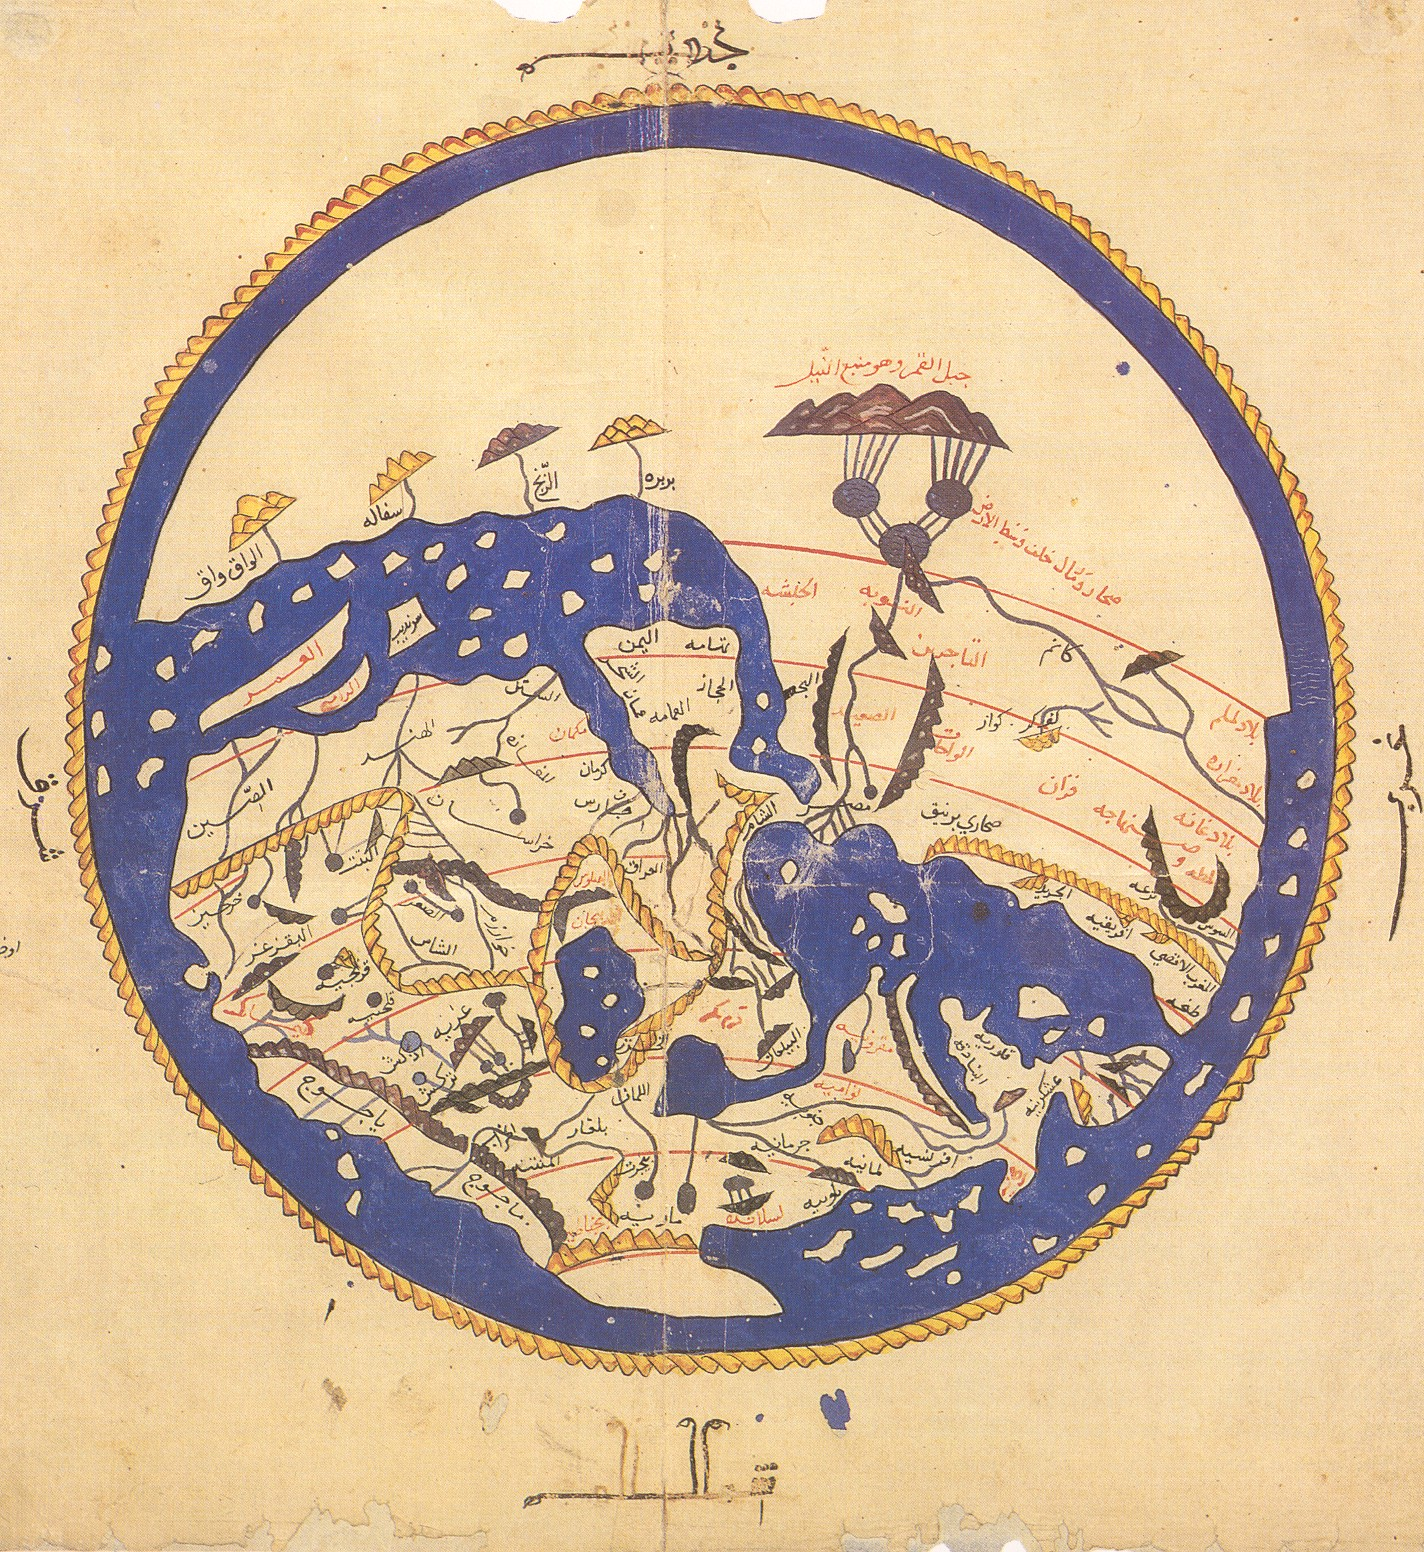
\includegraphics[width=1\textwidth]{figures/petaduniaalid.JPG}}
\caption{Gambaran pengantar peta dunia karya al-Idrisi tahun 1154.}
\end{figure}

\begin{figure}[ht]
	\centerline{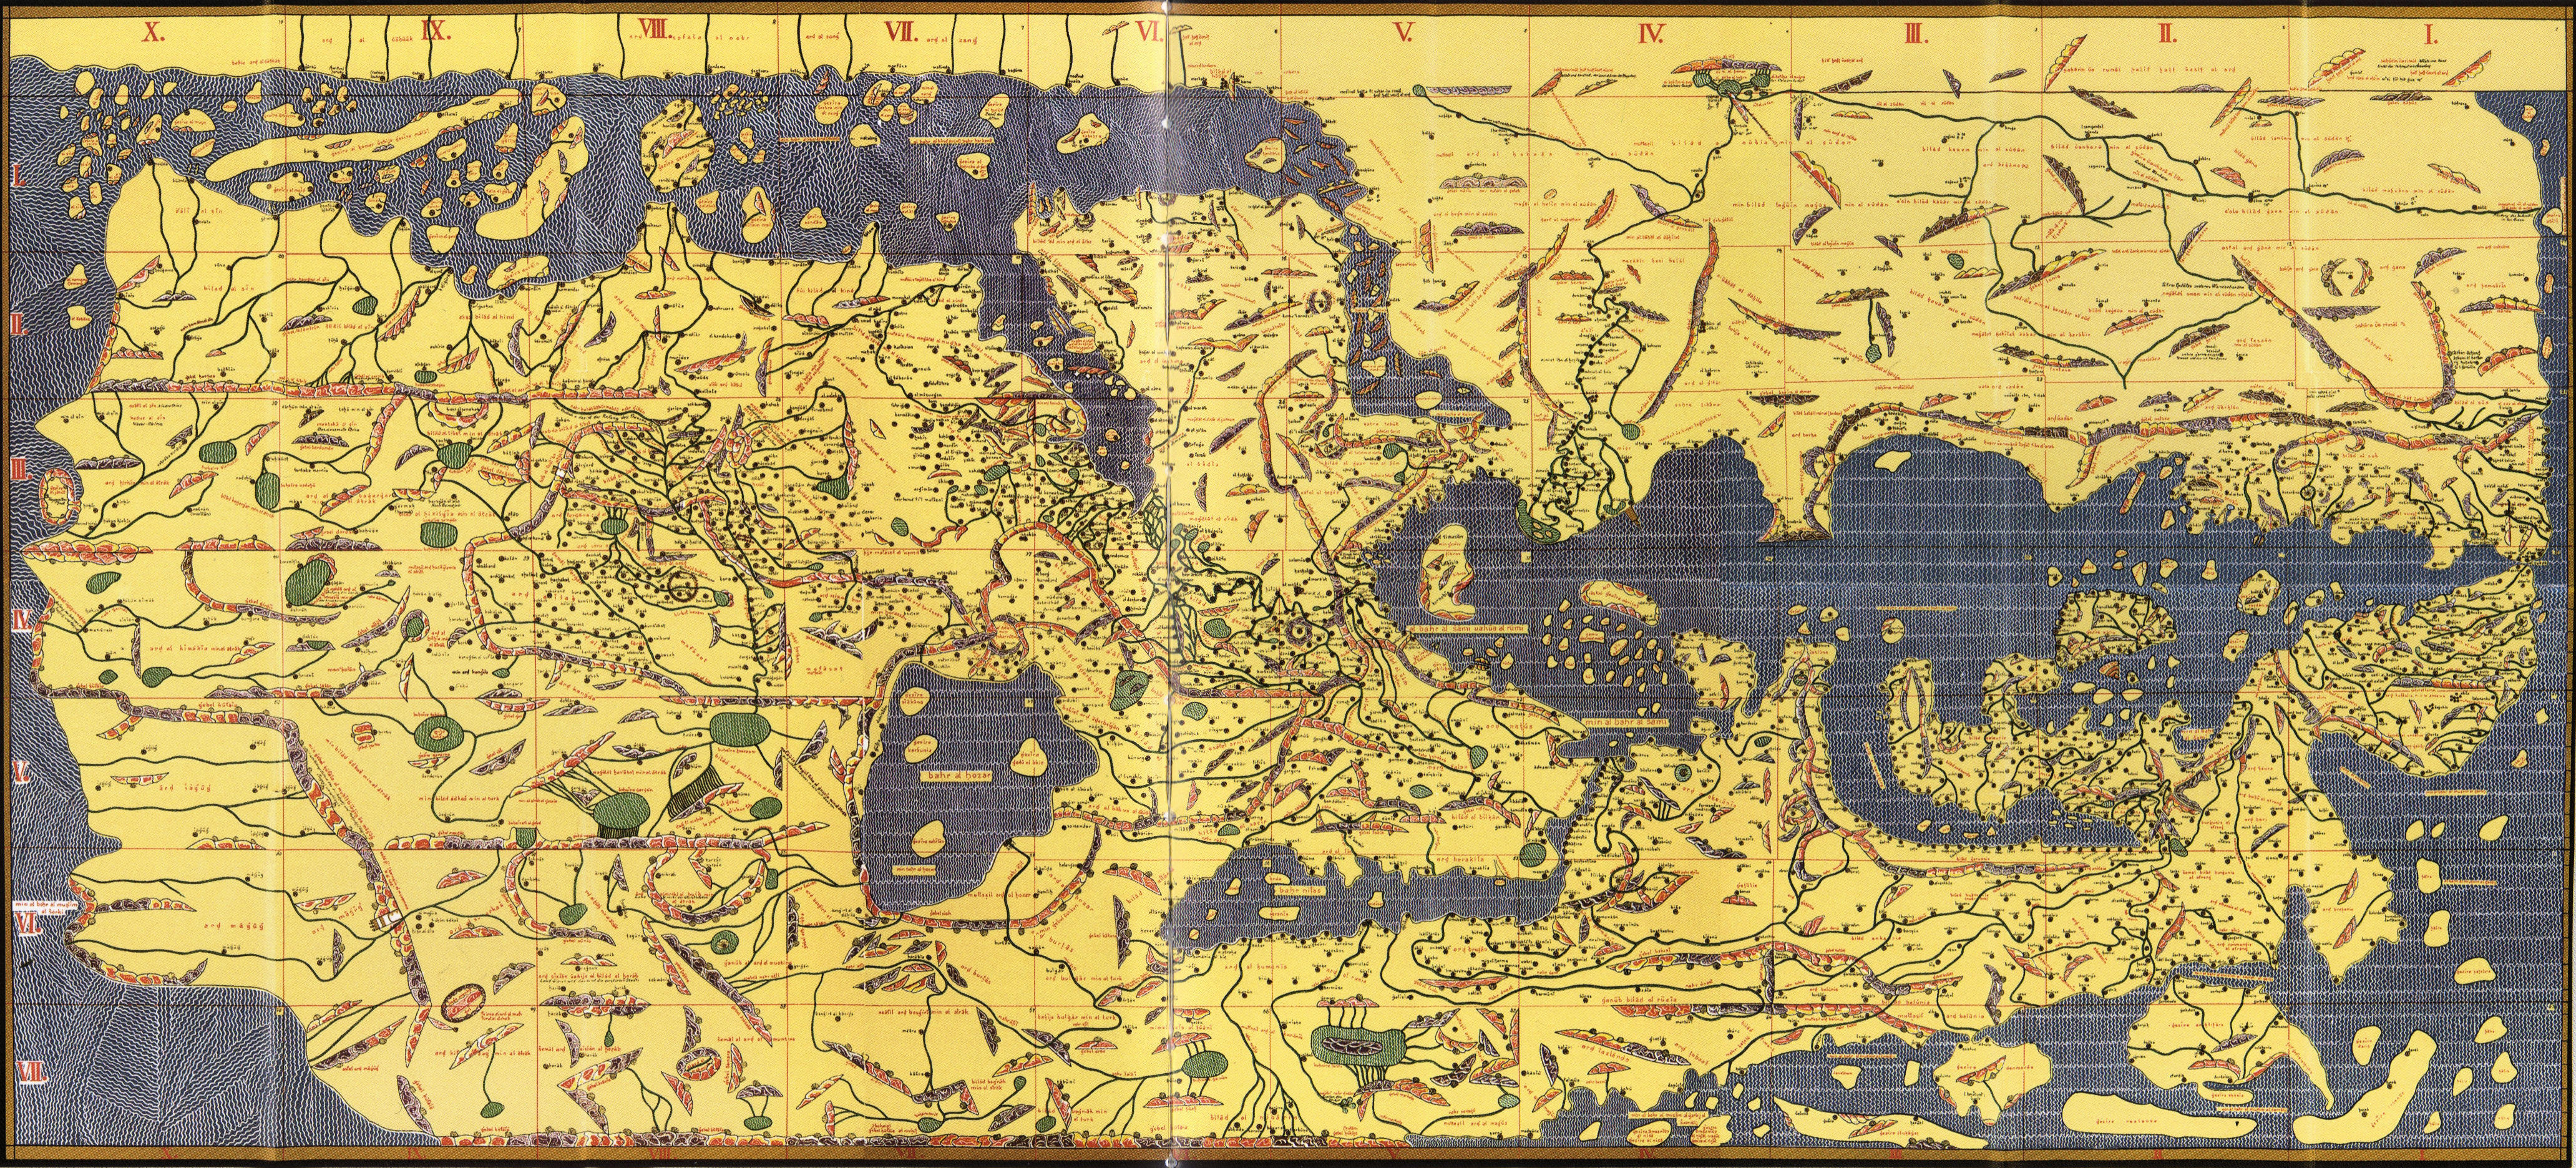
\includegraphics[width=1\textwidth]{figures/TabulaRogeriana.jpg}}
\vskip2pt
\caption{Tabula Rogeriana digambar oleh Al-Idrisi pada tahun 1154 untuk Raja Normandia Roger II dari Sisilia, setelah delapan menetap di istananya, di mana dia bekerja untuk penjelasan dan ilustrasi peta.}
\end{figure}

\section{Penentuan Kordinat}
Kordinat digunakan untuk mengacu sebuah titik lokasi di muka bumi, adapun beberapa jenis standar kordinat yang digunakan adalah.

\subsection{Kordinat Internasional}
Kordinat internasional dikenal dengan long dan lat.


\subsection{Kordinat Indonesia}
Masih ingatkah pelajaran geografi tentang letak Indonesia? maka kita bisa melihat jawaban tersebut dalam kordinat berbahasa indonesia.



\chapter[OS Semaphore]
{OS\\ Semaphore}
\section{System Operasi Semaphore}

	\subsection{Definisi}
	
		\begin{figure}[ht]
			\centerline{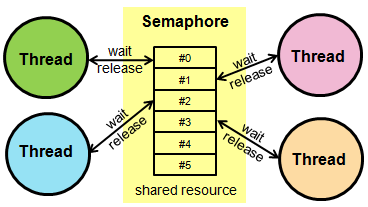
\includegraphics[width=0.5\textwidth]{figures/sema.png}}
			\caption{Semaphore}
			\label{sema}
			\end{figure}
	
		Semaphore merupakan salah satu teknik sinyal pada OS yang paling sederhana, dan merupakan konsep yang penting dalam OS desain, di mana nilai integer digunakan untuk memberi sinyal antar proses. 
		Hanya tiga operasi yang mungkin dilakukan pada semaphores, yang semuanya adalah atom: inisialisasi, keturunan, dan peningkatan. 
		Pengurangan operasi dapat menyebabkan proses yang diblokir, dan peningkatan operasi yang sedang berlangsung dapat mengakibatkan pemblokiran suatu proses. 
		Semaphore pada system operasi merupakan sebuah variabel bertipe integer. Di kehidupan nyata, semaphore merupakan sistem sinyal yang digunakan untuk memberi sinyal atau tanda dan berkomunikasi secara visual. 
		Semafor juga merupakan struktur data dalam bahasa komputer yang digunakan untuk menyinkronkan suatu proses, yaitu untuk memecahkan masalah di mana masalahnya lebih dari satu proses atau bisa 
		seperti thread yang akan dijalankan secara bersamaan dan harus diatur urutan kerja. Semaphore dibuat oleh Edsger Dijkstra dan pertama kali digunakan dalam sistem operasi.
		Nilai semaphore diinisialisasi dengan jumlah sumber daya yang dikontrol oleh pengguna. Dalam kasus khusus di mana ada sumber daya bersama, semaphore disebut semaphore biner. 
		Semaphore adalah solusi klasik dari dining philosophers problem, meskipun itu tidak mencegah deadlock.
		Pada software semaphore, semaphore merupakan variabel yang bertipe data integer tetapi tidak termasuk pada data yang sedang dilakukan inisialisasi, yang hanya dapat diakses melalui dua operasi standar, yaitu increment dan decrement. 
		Semaphore bisa digunakan untuk menyelesaikan masalah sinkronisasi secara umum, berdasarkan jenisnya. Semaphore hanya memiliki nilai 1 atau 0, atau lebih dari sama dengan 0. 
		Konsep semaphore pertama kali diajukan idenya oleh Edsger Dijkstra pada tahun 1967. Semaphore memiliki dua jenis, yaitu, Biner semaphore dan counting semaphore. 
		Biner semaphore tidak bisa memiliki semua jenis integer tetapi hanya memiliki 2 nilai yaitu 1 atau 0, Sering juga disebut sebagai semaphore primitive. Sedangkan Counting semaphore memiliki nilai 0, 1, sampai seterusnya atau integer lainnya. 
		Banyak sistem operasi yang tidak secara langsung menggunakan semaphore jenis ini, namun lebih banyak yang memanfaatkan semaphore jenis biner semaphore. 
		Pada semaphore ini harus diketahui bahwa, ada beberapa jenis dari counting semaphore yang salah satu jenisnya adalah semafor yang tidak bisa mencapai nilai negatif dan jenis yang lain adalah semaphore yang dapat mencapai nilai negatif. 
		Solusi dari Pembuatan Counting Semaphore adalah Binary Semaphore. Pembuatan counting semaphore banyak dilakukan para programmer untuk memenuhi alat sinkronisasi yang sesuai dengannya. 
		
		Operasi standarnya dalam bahasa pemrograman C :
		
		\begin{verbatim}
			void kunci(int sem_value) {
				while(sem_value <= 0);
				sem_value�;
			}
			void buka(int sem_value) {
				sem_value++;
			}
		\end{verbatim}
		
	\subsection{Prinsip Semaphore}
	
		\begin{enumerate}

			\item Suatu proses yang berbeda bisa berkaitan dengan memanfaatkan sinyal - sinyal.
			\item Suatu proses dapat dihentikan oleh proses yang lain.
			\item Semaphore bertipe data integer yang diakses oleh dua operasi atomik standar (wait dan signal).
			\item Ada dua operasi di semaphore (Down dan UP). Yang nama aslinya : P dan V.
		
		\end{enumerate}

	\subsection{Kelemahan Semaphore}
	
		\begin{enumerate}

			\item Semaphore termasuk Low Level.
			\item Dikarenakan semaphore tersebar di dalam seluruh program maka kita akan kesulitan dalam pemeliharaannya.
			\item Jika kita menghapus \"wait\" akan mengakibatkan \"nonmutual exclusion\".
			\item Jika kita menghapus \"signal\" akan mengakibatkan \"deadlock\".
			\item Jika terjadi deadlock akan sulit untuk dideteksi.

		\end{enumerate}
		
	\subsection{Semantik dan Impelementasi}
		Menghitung semaphores dilengkapi dengan dua operasi, secara historis dilambangkan sebagai P dan V (lihat § Nama operasi untuk nama alternatif). 
		Operasi V menambahkan semaphore S, dan operasi P menurunkannya.

		Nilai semaphore S adalah jumlah unit sumber daya yang saat ini tersedia. Operasi P membuang waktu atau tidur sampai sumber daya yang dilindungi oleh 
		semaphore menjadi tersedia, pada saat itu sumber daya segera diklaim. Operasi V adalah kebalikannya: ia membuat sumber daya tersedia lagi setelah proses
		selesai menggunakannya. Satu properti penting dari semaphore S adalah bahwa nilainya tidak dapat diubah kecuali dengan menggunakan operasi V dan P.

		Cara sederhana untuk memahami operasi tunggu (P) dan sinyal (V) adalah:
		
		\begin{itemize}
		
			\item menunggu: Jika nilai variabel semaphore tidak negatif, turunkan dengan 1. Jika variabel semaphore sekarang negatif, proses menunggu eksekusi 
			      diblokir (yaitu, ditambahkan ke antrian semaphore) sampai nilainya lebih besar atau sama dengan 1 Jika tidak, proses terus berjalan, setelah 
				  menggunakan satu unit sumber daya.
			\item sinyal: Menambah nilai semaphore variabel dengan 1. Setelah kenaikan, jika nilai pre-increment negatif (berarti ada proses menunggu sumber 
				  daya), ia mentransfer proses yang diblokir dari antrian menunggu semaphore ke antrean siap.
			
		\end{itemize}
		
		Banyak sistem operasi menyediakan primitif semaphore yang efisien yang membuka blokir proses menunggu ketika semaphore bertambah. Ini berarti bahwa proses tidak membuang waktu untuk memeriksa nilai semaphore yang tidak perlu.Konsep penghitungan semaphore dapat diperpanjang dengan kemampuan untuk mengklaim atau mengembalikan lebih dari satu \"unit\" dari semaphore, teknik yang diterapkan di Unix. Operasi V dan P yang dimodifikasi adalah sebagai berikut, menggunakan tanda kurung siku untuk menunjukkan operasi atom, yaitu operasi yang tampak terpisah dari perspektif proses lain:

		Semaphore pada system operasi merupakan sebuah variabel bertipe integer. Di kehidupan nyata, semaphore merupakan sistem sinyal yang digunakan untuk memberi sinyal atau tanda dan berkomunikasi secara visual. PPada software semaphore, semaphore merupakan variabel yang bertipe data integer tetapi tidak termasuk pada data yang sedang dilakukan inisialisasi, yang hanya dapat diakses melalui dua operasi standar, yaitu increment dan decrement. 
		Semaphore bisa digunakan untuk menyelesaikan masalah sinkronisasi secara umum, berdasarkan jenisnya. Semaphore hanya memiliki nilai 1 atau 0, atau lebih dari sama dengan 0. Konsep semaphore pertama kali diajukan idenya oleh Edsger Dijkstra pada tahun 1967. Semaphore memiliki dua jenis, yaitu, Biner semaphore dan counting semaphore. Biner semaphore hanya memiliki nilai 1 atau 0, Sering juga disebut sebagai semaphore primitive. Sedangkan Counting semaphore memiliki nilai 0, 1, sampai seterusnya atau integer lainnya. Banyak sistem operasi yang tidak secara langsung menggunakan semaphore jenis ini, namun lebih banyak yang memanfaatkan semaphore jenis biner semaphore

	
	\subsection{Prinsip Semaphore}
		\begin{enumerate}

			\item Suatu proses yang berbeda bisa berkaitan dengan memanfaatkan sinyal - sinyal.
			\item Suatu proses dapat dihentikan oleh proses lainnya.
			\item Semaphore bertipe data integer yang diakses oleh dua operasi atomik standar (wait dan signal).
			\item Ada dua operasi di semaphore (Down dan UP). Yang nama aslinya : P dan V.
			
		\end{enumerate}
		
	\subsection{Kelemahan Semaphore}

		\begin{enumerate}

			\item Semaphore termasuk Low Level.
			\item Dikarenaka semaphore tersebar di dalam seluruh program maka kita akan kesulitan dalam pemeliharaannya.
			\item Jika kita menghapus \"wait\" akan mengakibatkan \"nonmutual exclusion\".
			\item Jika kita menghapus \"signal\" akan mengakibatkan \"deadlock\".
			\item Jika terjadi deadlock akan sulti untuk dideteksi.
			
		\begin{enumerate}
		
	\cite{luu1982apparatus}
	\cite{lauesen1975large}
	\cite{hoare1974monitors}


\chapter[Proses OS]
{OS\\ Proses}
%kelompok 1 Sistem Operasi (Proses Os)
%Kelas D4 TI 1B
%Adam Noer Hidayatullah 1174097
%Ichsan Hizman
%Teddy
%Nisrina Aulia
%Irvan Rizkiansyah 1174043

\section{proses}

	\subsection{Proses}	
	Proses adalah sebuah  program yang sedang dieksekusi. Sedangkan program idalah merupakan kumpulan-kumpulan  dari suatu  instruksi yang sudah ditulis ke dalam bahasa yang dapat  dimengerti oleh sistem operasi.Proses berisi tentang sebuah instruksi dan sebuah data. program counter dan seluruh register pemroses, stack ini  berisi data sementara contohnya seperti alamat pengiriman, parameter rutin dan variabel lokal. Sistem operasi diharuskan untuk mengelola semua proses di dalam sistem tersebut dan mengalokasikan sumber daya ke sebuah  proses-proses sesuai dengan kebijaksanaan untuk memenuhi sasaran sistem
	
	\subsection{Istilah yang berkaitan dengan proses}
		\begin{itemize}
			\item Multiprogramming
			Multiprogramming (multitasking) adalah  istilah teknologi informasi dengan mengunakan bahasa inggris yang baik  mengacup kepada sebuah metode dimana banyak sebuah pekerjaan atau yang dikenal juga sebagai proses  dengan diolah dengan menggunakan sumber daya CPU yang sama.
			Contohnya sistem operasi jenis ini antaranya linux dan windows.
			\item Multiprocessing
			kemampuan komputer untuk melakukan beberapa proses dengan waktu yang bersamaan, dibantu dengan keberadaan teknologi yang berbasis multiprocessor.
			Contohnya seperti computer server.
			\item Distributed processing/computing
			Mengerjakan semua proses pengolahan data secara bersamaan antara komputer pusat dengan beberapa komputer yang lebih kecil dan saling berhubungan denan melalui jalur komunikasi.
			Contohnya komputer yang dirancang untuk melaksanakan tugas-tugas proyek.
		\end{itemize}
		
	\subsection{Fungsi fungsi sistem operasi}
		\begin{enumerate}
			\item Resource manager, pengolahan sumber daya dan mengalokasikan.
			\item Interface atau tatap muka, sebagai perantara antara pengguna dengan perangkat keras.
			\item Coordinator, mengkoordinasi fasilitas sehingga aktifitas yang komplek dapat diatur..
		\end{enumerate}
		
		\subsection{jenis jenis sistem operasi pada komputer}
			\begin{enumerate}
				\item Windows, merupakan pengembangan dari sistem operasi DOS. windows juga mudah untuk dipelajari.
				\item Mac OS, merupakan sistem operasi yang diciptakan oleh Apple. Mac OS memiliki tingkat keamanan yang tinggi.
				\item Linux, memiliki kestabilan yang baik, yang sering digunakan sebagai sistem operasi pada server.
				\item Android, merupakan sistem operasi pada smartphone. android sama seperti Linux, yaitu mudah dikembangkan.
			\end{enumerate}
			
	\subsection{Status proses}
	Terdapat 5 macam jenis status yang mungkin dimiliki oleh suatu proses :
	\begin{enumerate}
		\item New, yaitu status yang dimiliki pada saat proses baru saja terjadi.
		\item Ready, yaitu status dimana proses siap untuk dieksekusi pada giliran berikutnya.
		\item Running, yaitu status suatu proses dimana saat ini proses tersebut sedang dieksekusi oleh prosesor
		\item Waiting, yaitu status dimana proses yang tidak bisa dijalankan di saat prosesor sudah siap, status yang dimiliki pada saat proses menunggu suatu sebuah event seperti I/O
		\item Terminated, yaitu status yang dimiliki pada saat proses telah selesai dieksekusi
	\end{enumerate}
	
	Berikut ini adalah proses dari ke-5 status proses di atas :
	\begin{enumerate}
		\item New ke Ready
		Pertama Status dibuat lalu setelah itu , status akan memasuki proses ready dan siap untuk memasuki proses selanjutnya.
		\item Ready ke running
		Di saat sedang memilih proses yang akan dioperasikan, sistem operasi akan memilih salah satu proses yang berada didalam keadaan status ready.
		\item Running ke waiting
		Suatu proses dimasukkan dalam keadaan status waiting jika proses itu meminta sesuatu yang dapat menyebabkannya harus menunggu. Sebuah request ke sistem operasi yang pada umumnya merupakan bentuk panggilan dari layanan sistem (panggilan dari program yang sedang beroperasi ke dalam suatu prosedur yang merupakan bagian kode sistem operasi) misalnya seperti sebuah proses yang bisa meminta suatu layanan dari sistem operasi yang tidak siap dilakukan oleh sistem opersi dengan segera. Atau proses yang bisa menginisiasi suatu aksi, seperti misalnya operasi I/O, yang seharusnya bisa diselesaikan sebelum proses itu melanjutkan operasinya. Pada saat proses saling melakukan komunikasi dengan proses yang lainnya, suatu proses bisa diblokir jika sedang menunggu proses lainnya untuk menyediakan input.
		\item Running ke ready
		Pada umumnya alasan transisi ini ialah dimana sebuah proses yang lagi berjalan sudah mencapai batas waktu maksimum yang telah diizinkan bagi instruksi yang tidak diinterupsi. Terdapat beberapa alasan yang menyebabkan transisi ini terjadi, yang tidak diimplementasikan oleh setiap sistem operasi. Misalnya apabila sistem operasi meng-assign tingkat prioritas yang berbeda pada beberapa proses yang berlainan, suatu proses bisa diambil lebih dulu.
		\item Waiting ke ready
		Apabila suatu proses dalam keadaan status waiting sudah selesai dalam mendapatkan sumber daya, seperti file atau bagian virtual memori bagi pakai atau juga sudah selesai setelah menunggu proses yang lainnya untuk menyediakan input atau sudah selesai dalam menunggu pesan lainnya.
		\item Runing ke finish(terminated)
		proses yang sedang berjalan dihentikan oleh Sistem Operasi jika proses itu telah selesai atau tidak jadi dieksekusi. Hal ini terjadi dikarenakan jika proses induknya sendiri telah berhenti.
	\end{enumerate}
	
	Dan berikut ini adalah diagram dari ke-5 status proses tadi :
	
	\begin{figure} [ht]
	\centerline{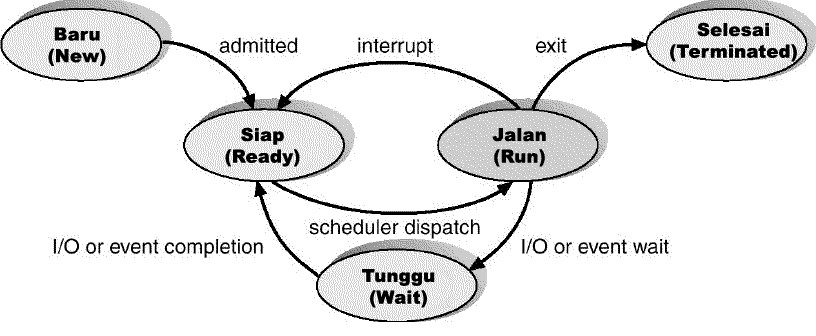
\includegraphics[width=1\textwidth]{figures/statusproses.jpg}}
	\caption{Gambar Status Proses}
	\label{statusproses}
	\end{figure}
	
	\ref{statusproses}
	
	\subsection{Contoh dari status proses}
	Setiap proses pasti mempunyai status yang harus diperhatikan oleh sistem operasi yang akan dicatat dalam berbagai macam tabel yang saling berhubungan, yaitu :
		\begin{itemize}
			\item Tabel informasi manajemen memori, Digunakan untuk menjaga keutuhan dari suatu memori utama dan memori sekunder yang akan menyimpan suatu informasi.
			\item Tabel informasi manajemen masukan atau keluaran, Digunakan untuk melakukan pengelolan sebuah perangkat masukan atau keluaran, yang dimana perangkat tersebut akan digunakan oleh proses yang tertentu, sehingga harus dijaga supaya proses yang lainnya tidak akan memakainya. Sistem operasi harus mengetahui status operasi masukan atau keluaran dan lokasi suatu memori utama yang akan digunakan untuk melakukan transfer data.
			\item Tabel informasi sistem file, Tabel dimana yang berisikan mengenai informasi lokasi pada memori sekunder, informasi ekstensi file, informasi status pada saat itu dan menyimpan atribut-atribut file yang lainnya.
			\item Tabel proses, Digunakan untuk mengelola informasi suatu proses pada sistem operasi, yang berlokasi di memori, atribut proses dan status lainnya.
		\end{itemize}
	
	\subsection{Proses Control Block/Blocked}
	Sebuah struktur data yang dipakai oleh Sistem Operasi untuk mengelola sebuah proses. Hampir semua Sistem Operasi yang modern telah menggunakan PCB (Process Control Block) namun strukturnya yang berbeda-beda pada setiap Sistem Operasi tersebut. PCB (Process Control Block) juga memiliki informasi yang berhubungan dengan proses, ialah: tanda pengenal bagi sebuah proses (Process ID) yang sangat unik dan akan menjadi status proses, nomor identitas, prioritas eksekusi proses dan semua informasi lokasi proses dalam memori. Prioritas yang dimiliki oleh sebuah proses merupakan sebuah nilai atau besaran yang akan menunjukkan seberapa sering proses harus dieksekusi oleh prosesor. Sebuah proses yang mempunyai nilai prioritas yang cenderung lebih tinggi, akan lebih sering dieksekusi atau dieksekusi terlebih dulu jika dibandingkan dengan proses yang mempunyai prioritas yang lebih rendah.
	Sebuah PCB (Process Control Block) ditunjukkan dalam tabel berikut : 
	
	\begin{table}[H]
		\begin{tabular}{|c|c|}
			\hline
			Pointer & State Proses\\
			\hline
			\multicolumn{2}{|c|}{Nomor Proses}\\
			\hline
			\multicolumn{2}{|c|}{Program Counter}\\
			\hline
			\multicolumn{2}{|c|}{Registers}\\
			\hline
			\multicolumn{2}{|c|}{Batas Memori}\\
			\hline
			\multicolumn{2}{|c|}{Daftar berkas yang telah dibuka}\\
			\hline
			\multicolumn{2}{|c|}{.......}\\
		\end{tabular}
	\end{table}
	
	PCB dibagi menjadi 3 kelompok yaitu :
	\begin{itemize}
		\item Process identification data
		pasti akan selalu mengikut-sertakan suatu identifier yang sangat unik untuk prosesnya (hampir selalu mempunyai nilai integer) dan pada sebuah sistem multiuser-multitasking, data yang contohnya seperti identifier grup pengguna, identifier proses, identifier pengguna, dan yang lainnya. Proses ini sangat relevan, karena itu sering dipakai untuk referensi silang tabel sistem operasi, misalnya seperti memungkinkan untuk mengidentifikasi sebuah proses yang menggunakan device I/O, atau daerah memori.
		\item Processor state data
		potongan-potongan dari informasi yang mengartidefinisikan status dari sebuah proses ketika proses tersebut ditangguhkan, dan memungkinkan sistem operasi untuk melakukan restart proses pada akhirnya dan akan masih dapat mengeksekusinya dengan benar. Hal ini akan selalu mengikut-sertakan isi dari register CPU tujuan.
		\item Process control data
		digunakan oleh sistem operasi untuk mengelola proses itu sendiri.
	\end{itemize}
Dirangkum dari makalah \cite{apriyanto2009sistem}
Dirangkum dari makalah \cite{silberschatz2014operating}

{OS\\ Proses OS}
%kelompok 1 Sistem Operasi (Proses Os)
%Kelas D4 TI 1B
%Adam Noer Hidayatullah 1174097
%Ichsan Hizman
%Teddy
%Nisrina Aulia
%Irvan Rizkiansyah 1174043

\section{proses}

	\subsection{Proses}	
	Proses adalah sebuah  program yang sedang dieksekusi. Sedangkan program idalah merupakan kumpulan-kumpulan  dari suatu  instruksi yang sudah ditulis ke dalam bahasa yang dapat  dimengerti oleh sistem operasi.Proses berisi tentang sebuah instruksi dan sebuah data. program counter dan seluruh register pemroses, stack ini  berisi data sementara contohnya seperti alamat pengiriman, parameter rutin dan variabel lokal. Sistem operasi diharuskan untuk mengelola semua proses di dalam sistem tersebut dan mengalokasikan sumber daya ke sebuah  proses-proses sesuai dengan kebijaksanaan untuk memenuhi sasaran sistem
	
	\subsection{Istilah yang berkaitan dengan proses}
		\begin{itemize}
			\item Multiprogramming
			Multiprogramming (multitasking) adalah  istilah teknologi informasi dengan mengunakan bahasa inggris yang baik  mengacup kepada sebuah metode dimana banyak sebuah pekerjaan atau yang dikenal juga sebagai proses  dengan diolah dengan menggunakan sumber daya CPU yang sama.
			Contohnya sistem operasi jenis ini antaranya linux dan windows.
			\item Multiprocessing
			kemampuan komputer untuk melakukan beberapa proses dengan waktu yang bersamaan, dibantu dengan keberadaan teknologi yang berbasis multiprocessor.
			Contohnya seperti computer server.
			\item Distributed processing/computing
			Mengerjakan semua proses pengolahan data secara bersamaan antara komputer pusat dengan beberapa komputer yang lebih kecil dan saling berhubungan denan melalui jalur komunikasi.
			Contohnya komputer yang dirancang untuk melaksanakan tugas-tugas proyek.
		\end{itemize}
		
	\subsection{Fungsi fungsi sistem operasi}
		\begin{enumerate}
			\item Resource manager, pengolahan sumber daya dan mengalokasikan.
			\item Interface atau tatap muka, sebagai perantara antara pengguna dengan perangkat keras.
			\item Coordinator, mengkoordinasi fasilitas sehingga aktifitas yang komplek dapat diatur..
		\end{enumerate}
		
		\subsection{jenis jenis sistem operasi pada komputer}
			\begin{enumerate}
				\item Windows, merupakan pengembangan dari sistem operasi DOS. windows juga mudah untuk dipelajari.
				\item Mac OS, merupakan sistem operasi yang diciptakan oleh Apple. Mac OS memiliki tingkat keamanan yang tinggi.
				\item Linux, memiliki kestabilan yang baik, yang sering digunakan sebagai sistem operasi pada server.
				\item Android, merupakan sistem operasi pada smartphone. android sama seperti Linux, yaitu mudah dikembangkan.
			\end{enumerate}
			
	\subsection{Status proses}
	Terdapat 5 macam jenis status yang mungkin dimiliki oleh suatu proses :
	\begin{enumerate}
		\item New, yaitu status yang dimiliki pada saat proses baru saja terjadi.
		\item Ready, yaitu status dimana proses siap untuk dieksekusi pada giliran berikutnya.
		\item Running, yaitu status suatu proses dimana saat ini proses tersebut sedang dieksekusi oleh prosesor
		\item Waiting, yaitu status dimana proses yang tidak bisa dijalankan di saat prosesor sudah siap, status yang dimiliki pada saat proses menunggu suatu sebuah event seperti I/O
		\item Terminated, yaitu status yang dimiliki pada saat proses telah selesai dieksekusi
	\end{enumerate}
	
	Berikut ini adalah proses dari ke-5 status proses di atas :
	\begin{enumerate}
		\item New ke Ready
		Pertama Status dibuat lalu setelah itu , status akan memasuki proses ready dan siap untuk memasuki proses selanjutnya.
		\item Ready ke running
		Di saat sedang memilih proses yang akan dioperasikan, sistem operasi akan memilih salah satu proses yang berada didalam keadaan status ready.
		\item Running ke waiting
		Suatu proses dimasukkan dalam keadaan status waiting jika proses itu meminta sesuatu yang dapat menyebabkannya harus menunggu. Sebuah request ke sistem operasi yang pada umumnya merupakan bentuk panggilan dari layanan sistem (panggilan dari program yang sedang beroperasi ke dalam suatu prosedur yang merupakan bagian kode sistem operasi) misalnya seperti sebuah proses yang bisa meminta suatu layanan dari sistem operasi yang tidak siap dilakukan oleh sistem opersi dengan segera. Atau proses yang bisa menginisiasi suatu aksi, seperti misalnya operasi I/O, yang seharusnya bisa diselesaikan sebelum proses itu melanjutkan operasinya. Pada saat proses saling melakukan komunikasi dengan proses yang lainnya, suatu proses bisa diblokir jika sedang menunggu proses lainnya untuk menyediakan input.
		\item Running ke ready
		Pada umumnya alasan transisi ini ialah dimana sebuah proses yang lagi berjalan sudah mencapai batas waktu maksimum yang telah diizinkan bagi instruksi yang tidak diinterupsi. Terdapat beberapa alasan yang menyebabkan transisi ini terjadi, yang tidak diimplementasikan oleh setiap sistem operasi. Misalnya apabila sistem operasi meng-assign tingkat prioritas yang berbeda pada beberapa proses yang berlainan, suatu proses bisa diambil lebih dulu.
		\item Waiting ke ready
		Apabila suatu proses dalam keadaan status waiting sudah selesai dalam mendapatkan sumber daya, seperti file atau bagian virtual memori bagi pakai atau juga sudah selesai setelah menunggu proses yang lainnya untuk menyediakan input atau sudah selesai dalam menunggu pesan lainnya.
		\item Runing ke finish(terminated)
		proses yang sedang berjalan dihentikan oleh Sistem Operasi jika proses itu telah selesai atau tidak jadi dieksekusi. Hal ini terjadi dikarenakan jika proses induknya sendiri telah berhenti.
	\end{enumerate}
	
	Dan berikut ini adalah diagram dari ke-5 status proses tadi :
	
	\begin{figure} [ht]
	\centerline{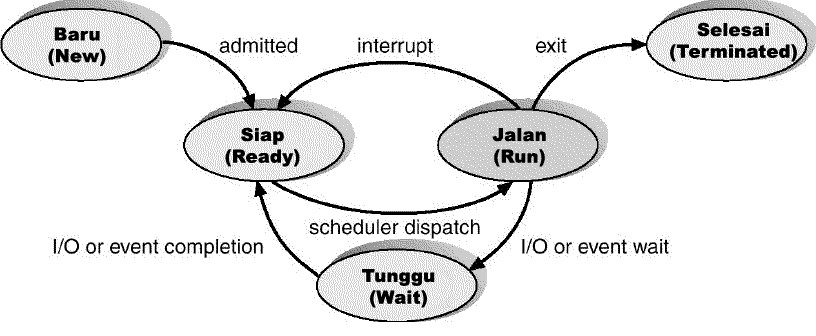
\includegraphics[width=1\textwidth]{figures/statusproses.jpg}}
	\caption{Gambar Status Proses}
	\label{statusproses}
	\end{figure}
	
	\ref{statusproses}
	
	\subsection{Contoh dari status proses}
	Setiap proses pasti mempunyai status yang harus diperhatikan oleh sistem operasi yang akan dicatat dalam berbagai macam tabel yang saling berhubungan, yaitu :
		\begin{itemize}
			\item Tabel informasi manajemen memori, Digunakan untuk menjaga keutuhan dari suatu memori utama dan memori sekunder yang akan menyimpan suatu informasi.
			\item Tabel informasi manajemen masukan atau keluaran, Digunakan untuk melakukan pengelolan sebuah perangkat masukan atau keluaran, yang dimana perangkat tersebut akan digunakan oleh proses yang tertentu, sehingga harus dijaga supaya proses yang lainnya tidak akan memakainya. Sistem operasi harus mengetahui status operasi masukan atau keluaran dan lokasi suatu memori utama yang akan digunakan untuk melakukan transfer data.
			\item Tabel informasi sistem file, Tabel dimana yang berisikan mengenai informasi lokasi pada memori sekunder, informasi ekstensi file, informasi status pada saat itu dan menyimpan atribut-atribut file yang lainnya.
			\item Tabel proses, Digunakan untuk mengelola informasi suatu proses pada sistem operasi, yang berlokasi di memori, atribut proses dan status lainnya.
		\end{itemize}
	
	\subsection{Proses Control Block/Blocked}
	Sebuah struktur data yang dipakai oleh Sistem Operasi untuk mengelola sebuah proses. Hampir semua Sistem Operasi yang modern telah menggunakan PCB (Process Control Block) namun strukturnya yang berbeda-beda pada setiap Sistem Operasi tersebut. PCB (Process Control Block) juga memiliki informasi yang berhubungan dengan proses, ialah: tanda pengenal bagi sebuah proses (Process ID) yang sangat unik dan akan menjadi status proses, nomor identitas, prioritas eksekusi proses dan semua informasi lokasi proses dalam memori. Prioritas yang dimiliki oleh sebuah proses merupakan sebuah nilai atau besaran yang akan menunjukkan seberapa sering proses harus dieksekusi oleh prosesor. Sebuah proses yang mempunyai nilai prioritas yang cenderung lebih tinggi, akan lebih sering dieksekusi atau dieksekusi terlebih dulu jika dibandingkan dengan proses yang mempunyai prioritas yang lebih rendah.
	Sebuah PCB (Process Control Block) ditunjukkan dalam tabel berikut : 
	
	\begin{table}[H]
		\begin{tabular}{|c|c|}
			\hline
			Pointer & State Proses\\
			\hline
			\multicolumn{2}{|c|}{Nomor Proses}\\
			\hline
			\multicolumn{2}{|c|}{Program Counter}\\
			\hline
			\multicolumn{2}{|c|}{Registers}\\
			\hline
			\multicolumn{2}{|c|}{Batas Memori}\\
			\hline
			\multicolumn{2}{|c|}{Daftar berkas yang telah dibuka}\\
			\hline
			\multicolumn{2}{|c|}{.......}\\
		\end{tabular}
	\end{table}
	
	PCB dibagi menjadi 3 kelompok yaitu :
	\begin{itemize}
		\item Process identification data
		pasti akan selalu mengikut-sertakan suatu identifier yang sangat unik untuk prosesnya (hampir selalu mempunyai nilai integer) dan pada sebuah sistem multiuser-multitasking, data yang contohnya seperti identifier grup pengguna, identifier proses, identifier pengguna, dan yang lainnya. Proses ini sangat relevan, karena itu sering dipakai untuk referensi silang tabel sistem operasi, misalnya seperti memungkinkan untuk mengidentifikasi sebuah proses yang menggunakan device I/O, atau daerah memori.
		\item Processor state data
		potongan-potongan dari informasi yang mengartidefinisikan status dari sebuah proses ketika proses tersebut ditangguhkan, dan memungkinkan sistem operasi untuk melakukan restart proses pada akhirnya dan akan masih dapat mengeksekusinya dengan benar. Hal ini akan selalu mengikut-sertakan isi dari register CPU tujuan.
		\item Process control data
		digunakan oleh sistem operasi untuk mengelola proses itu sendiri.
	\end{itemize}
Dirangkum dari makalah \cite{apriyanto2009sistem}
Dirangkum dari makalah \cite{silberschatz2014operating}

\chapter[Sistem Operasi]
{OS\\ Sistem Operasi}
\section{Sistem Operasi}
	\subsection{Definisi}
		\begin{enumerate}
			\item Sistem operasi (OS) adalah sistem perangkat lunak yang mengelola hardware dan sumber daya perangkat lunak dengan menyediakan pelayanan secara umum untuk program komputer.

			\item Sistem operasi berbagi waktu menjadwalkan tugas untuk penggunaan sistem yang efisien dan mungkin juga termasuk perangkat lunak akuntansi untuk alokasi biaya waktu prosesor, penyimpanan massal, pencetakan, dan sumber daya lainnya.
			\item Untuk fungsi perangkat keras seperti input dan output dan alokasi memori, sistem operasi bertindak sebagai perantara antara program dan perangkat keras komputer, meskipun kode aplikasi biasanya dijalankan langsung oleh perangkat keras dan sering membuat panggilan sistem ke fungsi OS atau terganggu oleh saya t. Sistem operasi banyak ditemukan pada perangkat komputer,telepon seluler dan konsol permainan video ke server web dan superkomputer.

			\item Sistem operasi berbagi waktu menjadwalkan tugas untuk penggunaan sistem yang efisien dan mungkin juga termasuk perangkat lunak akuntansi untuk alokasi biaya waktu prosesor, penyimpanan massal, pencetakan, dan sumber daya lainnya.
			\item Untuk fungsi perangkat keras seperti input dan output dan alokasi memori, sistem operasi bertindak sebagai perantara antara program dan perangkat keras komputer, meskipun kode aplikasi biasanya dijalankan langsung oleh perangkat keras dan sering membuat panggilan sistem ke fungsi OS atau terganggu oleh saya t. Sistem operasi banyak ditemukan pada perangkat komputer,telepon seluler dan konsol permainan video ke server web dan superkomputer.

			\item Sistem operasi desktop yang dominan adalah Microsoft Windows dengan pangsa pasar sekitar 82,74%. macOS oleh Apple Inc. berada di tempat kedua (13,23%), dan varietas Linux secara kolektif berada di tempat ketiga (1,57%). Di sektor seluler (gabungan ponsel dan tablet), penggunaan pada tahun 2017 adalah hingga 70% dari Google Android dan menurut data kuartal ketiga 2016, Android pada smartphone dominan dengan 87,5 persen dan tingkat pertumbuhan 10,3 persen per tahun, diikuti oleh Apple iOS dengan 12,1 persen dan penurunan per tahun di pangsa pasar 5,2 persen, sementara jumlah sistem operasi lainnya hanya 0,3 persen. Distribusi Linux dominan di sektor server dan superkomputer. Kelas khusus lainnya dari sistem operasi, seperti embedded dan sistem real-time, ada untuk banyak aplikasi.
		\end{enumerate}
	\begin{figure}[ht]
		\centerline{
\includegraphics[width=1\textwidth]{figures/OS.JPG}}
		\caption{Sistem Operasi}
		\label{OS}
	\end{figure}

\subsection{Jenis sistem operasi}
\subsubsection{Single dan multi-tasking}
	\begin{enumerate}
		\item Sistem satu tugas hanya dapat menjalankan satu program dalam satu waktu, sementara sistem operasi multi-tasking memungkinkan lebih dari satu program berjalan dalam konkurensi. Ini dicapai dengan time-sharing, di mana waktu prosesor yang tersedia dibagi antara beberapa proses. Proses ini masing-masing terganggu berulang kali dalam irisan waktu oleh subsistem penjadwalan tugas dari sistem operasi. Multi-tasking dapat dicirikan dalam tipe preemptif dan kooperatif. Dalam preemptive multitasking, sistem operasi memotong waktu CPU dan mendedikasikan slot untuk masing-masing program. Sistem operasi mirip Unix, seperti Solaris dan Linux — serta non-Unix-like, seperti AmigaOS — mendukung multitasking preemptif. Multitasking kooperatif dicapai dengan mengandalkan pada setiap proses untuk menyediakan waktu untuk proses lain dengan cara yang ditentukan. Versi 16-bit Microsoft Windows menggunakan multi-tasking kooperatif. Versi 32-bit dari Windows NT dan Win9x, menggunakan preemptive multi-tasking.
	\end{enumerate}
\subsection{Single dan multi-user}
	\begin{enumerate}
		\item 1. Sistem operasi pengguna tunggal tidak memiliki fasilitas untuk membedakan pengguna, tetapi dapat memungkinkan beberapa program berjalan bersama-sama. Sistem operasi multi-pengguna memperluas konsep dasar multi-tasking dengan fasilitas yang mengidentifikasi proses dan sumber daya, seperti ruang disk, milik beberapa pengguna, dan sistem memungkinkan banyak pengguna untuk berinteraksi dengan sistem pada saat yang bersamaan. 
		\item 2. Sistem operasi berbagi waktu menjadwalkan tugas untuk penggunaan sistem yang efisien dan mungkin juga termasuk perangkat lunak akuntansi untuk alokasi biaya waktu prosesor, penyimpanan massal, pencetakan, dan sumber daya lainnya untuk banyak pengguna.
	\end{enumerate}
\subsection{Pendistribusian}
	\begin{enumerate}
		\item Sistem operasi terdistribusi mengelola sekelompok komputer yang berbeda dan membuatnya tampak sebagai komputer tunggal. Pengembangan jaringan komputer yang dapat dihubungkan dan berkomunikasi satu sama lain menimbulkan komputasi terdistribusi. Komputasi terdistribusi dilakukan pada lebih dari satu mesin. Ketika komputer dalam kelompok bekerja dalam kerja sama, mereka membentuk sistem terdistribusi.
	\end{enumerate}
\subsection{Sejarah}
	\begin{enumerate}
		\item Komputer awal dibangun untuk melakukan serangkaian tugas tunggal, seperti kalkulator. Fitur-fitur sistem operasi dasar dikembangkan pada tahun 1950-an, seperti fungsi monitor penduduk yang dapat secara otomatis menjalankan program yang berbeda secara berurutan untuk mempercepat pemrosesan. Sistem operasi tidak ada dalam bentuk modern dan lebih kompleks hingga awal 1960-an. Fitur perangkat keras ditambahkan, yang memungkinkan penggunaan pustaka runtime, interupsi, dan pemrosesan paralel. Ketika komputer pribadi menjadi populer pada tahun 1980-an, sistem operasi dibuat untuk mereka yang serupa dalam konsep untuk yang digunakan pada komputer yang lebih besar.

		\item Pada 1940-an, sistem digital elektronik paling awal tidak memiliki sistem operasi. Sistem elektronik saat ini diprogram pada deretan switch mekanis atau oleh kabel jumper pada papan steker. Ini adalah sistem tujuan khusus yang, misalnya, menghasilkan tabel balistik untuk militer atau mengontrol pencetakan cek gaji dari data pada kartu kertas berlubang. Setelah komputer tujuan umum yang dapat diprogram diciptakan, bahasa mesin (terdiri dari string digit biner 0 dan 1 pada pita kertas berlubang) diperkenalkan yang mempercepat proses pemrograman.
		\item Pada awal 1950-an, komputer hanya dapat menjalankan satu program dalam satu waktu. Setiap pengguna memiliki satu-satunya penggunaan komputer untuk jangka waktu terbatas dan akan tiba pada waktu yang dijadwalkan dengan program dan data pada kartu kertas berlubang atau pita berlubang. Program akan dimuat ke dalam mesin, dan mesin akan diatur untuk bekerja sampai program selesai atau crash. Program umumnya dapat di-debug melalui panel depan menggunakan saklar beralih dan lampu panel. Dikatakan bahwa Alan Turing adalah seorang ahli dalam mesin Manchester Mark 1 awal ini, dan dia sudah mendapatkan konsep primitif dari sistem operasi dari prinsip-prinsip mesin Turing universal.
		\item Kemudian mesin datang dengan perpustakaan program, yang akan dikaitkan dengan program pengguna untuk membantu dalam operasi seperti input dan output dan menghasilkan kode komputer dari kode simbolik yang dapat dibaca manusia. Ini adalah awal dari sistem operasi modern. Namun, mesin masih menjalankan pekerjaan tunggal pada suatu waktu. Di Cambridge University di Inggris, antrian pekerjaan pada suatu waktu adalah garis pencucian (garis pakaian) dari mana kaset digantung dengan pakaian warna berbeda untuk menunjukkan prioritas pekerjaan. 

		\item Pada 1940-an, sistem digital elektronik paling awal tidak memiliki sistem operasi. Sistem elektronik saat ini diprogram pada deretan switch mekanis atau oleh kabel jumper pada papan steker. Ini adalah sistem tujuan khusus yang, misalnya, menghasilkan tabel balistik untuk militer atau mengontrol pencetakan cek gaji dari data pada kartu kertas berlubang. Setelah komputer tujuan umum yang dapat diprogram diciptakan, bahasa mesin (terdiri dari string digit biner 0 dan 1 pada pita kertas berlubang) diperkenalkan yang mempercepat proses pemrograman.
		\item Pada awal 1950-an, komputer hanya dapat menjalankan satu program dalam satu waktu. Setiap pengguna memiliki satu-satunya penggunaan komputer untuk jangka waktu terbatas dan akan tiba pada waktu yang dijadwalkan dengan program dan data pada kartu kertas berlubang atau pita berlubang. Program akan dimuat ke dalam mesin, dan mesin akan diatur untuk bekerja sampai program selesai atau crash. Program umumnya dapat di-debug melalui panel depan menggunakan saklar beralih dan lampu panel. Dikatakan bahwa Alan Turing adalah seorang ahli dalam mesin Manchester Mark 1 awal ini, dan dia sudah mendapatkan konsep primitif dari sistem operasi dari prinsip-prinsip mesin Turing universal.
		\item Kemudian mesin datang dengan perpustakaan program, yang akan dikaitkan dengan program pengguna untuk membantu dalam operasi seperti input dan output dan menghasilkan kode komputer dari kode simbolik yang dapat dibaca manusia. Ini adalah awal dari sistem operasi modern. Namun, mesin masih menjalankan pekerjaan tunggal pada suatu waktu. Di Cambridge University di Inggris, antrian pekerjaan pada suatu waktu adalah garis pencucian (garis pakaian) dari mana kaset digantung dengan pakaian warna berbeda untuk menunjukkan prioritas pekerjaan. 

	\end{enumerate}
\subsection{Mikrokomputer}
	\begin{enumerate}
		\item Mikrokomputer pertama tidak memiliki kapasitas atau kebutuhan untuk sistem operasi yang rumit yang telah dikembangkan untuk mainframe dan miniis, sistem operasi minimalis dikembangkan, sering dimuat dari ROM dan dikenal sebagai monitor. Salah satu sistem operasi disk awal yang terkenal adalah CP / M, yang didukung oleh banyak mikrokomputer awal dan sangat ditiru oleh Microsoft MS-DOS, yang menjadi sangat populer sebagai sistem operasi yang dipilih untuk PC IBM . Pada 1980-an, Apple Computer Inc.  meninggalkan seri mikrokomputer Apple II yang populer untuk memperkenalkan komputer Apple Macintosh dengan antarmuka pengguna grafis inovatif  ke Mac OS.

		\item Pengenalan chip CPU Intel 80386 pada bulan Oktober 1985,  dengan arsitektur 32-bit dan kemampuan paging, menyediakan komputer pribadi dengan kemampuan untuk menjalankan sistem operasi multitasking seperti komputer minikomputer dan mainframe sebelumnya. Microsoft merespon perkembangan ini dengan mempekerjakan Dave Cutler, yang telah mengembangkan sistem operasi VMS untuk Digital Equipment Corporation. Dia dijadikan pemimpin dalam proses  pengembangan sistem operasi Windows NT, yang terus-menerus berfungsi sebagai dasar untuk jalur/way sistem operasi Microsoft. Steve Jobs, co-founder Apple Inc., memulai NeXT Computer Inc., yang mengembangkan sistem operasi NEXTSTEP. NEXTSTEP nantinya akan diakuisisi oleh Apple Inc. dan digunakan, bersama dengan kode dari FreeBSD sebagai inti dari Mac OS X.

		\item Pengenalan chip CPU Intel 80386 pada bulan Oktober 1985,  dengan arsitektur 32-bit dan kemampuan paging, menyediakan komputer pribadi dengan kemampuan untuk menjalankan sistem operasi multitasking seperti komputer minikomputer dan mainframe sebelumnya. Microsoft merespon perkembangan ini dengan mempekerjakan Dave Cutler, yang telah mengembangkan sistem operasi VMS untuk Digital Equipment Corporation. Dia dijadikan pemimpin dalam proses  pengembangan sistem operasi Windows NT, yang terus-menerus berfungsi sebagai dasar untuk jalur/way sistem operasi Microsoft. Steve Jobs, co-founder Apple Inc., memulai NeXT Computer Inc., yang mengembangkan sistem operasi NEXTSTEP. NEXTSTEP nantinya akan diakuisisi oleh Apple Inc. dan digunakan, bersama dengan kode dari FreeBSD sebagai inti dari Mac OS X.

		\item Proyek GNU dimulai oleh aktivis dan programmer Richard Stallman dengan tujuan menciptakan penggantian perangkat lunak gratis yang lengkap ke sistem operasi UNIX yang berpemilik. Meskipun proyek ini sangat berhasil dalam menduplikasi fungsionalitas berbagai bagian UNIX, pengembangan kernel GNU Hurd terbukti tidak produktif. Pada tahun 1991, mahasiswa ilmu komputer Finlandia Linus Torvalds, dengan kerja sama dari sukarelawan yang berkolaborasi melalui Internet, merilis versi pertama dari kernel Linux. Itu segera bergabung dengan komponen ruang pengguna GNU dan perangkat lunak sistem untuk membentuk sistem operasi yang lengkap. Sejak itu, kombinasi dari dua komponen utama biasanya hanya disebut Linux oleh industri perangkat lunak, konvensi penamaan yang Stallman dan Free Software Foundation tetap lawan, lebih memilih nama GNU / Linux. Berkeley Software Distribution, adalah bagian dari UNIX yang dirancang oleh University of California, Berkeley, dimulai pada thn 1970-an. Di distribusikan secara bebas dan diberikan ke banyak minikomputer, akhirnyapun mereka  memperoleh pengikut untuk digunakan pada PC, terutama sebagai FreeBSD, NetBSD dan OpenBSD.
	\end{enumerate}
\subsection{Berkeley Software Distribution}
	\begin{enumerate}
		\item Subkelompok keluarga Unix adalah keluarga Distribusi Perangkat Lunak Berkeley, yang mencakup FreeBSD, NetBSD, dan OpenBSD. Sistem operasi ini paling sering ditemukan di webservers, meskipun mereka juga dapat berfungsi sebagai OS komputer pribadi. Internet berutang banyak Kebijaksanaan untuk BSD, karena banyak dari protokol sekarang digunakan oleh komputer untuk menghubungkan, mengirim dan menerima data melalui jaringan diimplementasikan dan disempurnakan di BSD. World Wide Web Juga pertama kali dilakukan pada komputer yang menjalankan OS berdasarkan BSD yang disebut NeXTSTEP.

		\item Pada tahun 1974, University of California, Berkeley menciptakan sistem Unix awal. Seiring waktu, mahasiswa dan staf di departemen ilmu komputer telah mulai menambahkan program baru untuk menyederhanakan, seperti editor teks. Ketika Berkeley menerima komputer VAX baru pada tahun 1978 dengan Unixempat, para siswa di sekolah berbakat Unix lebih banyak menggunakan perangkat keras komputer. Departemen Pertahanan Advanced Defense Agency tertarik, dan memutuskan untuk mendanai proyek tersebut. Banyak sekolah, perusahaan, dan organisasi pemerintah menggunakan versi Berkeley dari Unix dan bukan yang resmi yang digunakan oleh AT dan T.

		\item Pada tahun 1974, University of California, Berkeley menciptakan sistem Unix awal. Seiring waktu, mahasiswa dan staf di departemen ilmu komputer telah mulai menambahkan program baru untuk menyederhanakan, seperti editor teks. Ketika Berkeley menerima komputer VAX baru pada tahun 1978 dengan Unixempat, para siswa di sekolah berbakat Unix lebih banyak menggunakan perangkat keras komputer. Departemen Pertahanan Advanced Defense Agency tertarik, dan memutuskan untuk mendanai proyek tersebut. Banyak sekolah, perusahaan, dan organisasi pemerintah menggunakan versi Berkeley dari Unix dan bukan yang resmi yang digunakan oleh AT dan T.

		\item Steve Jobs, setelah Apple Inc. pada tahun 1985, membentuk NeXT Inc., perusahaan yang memproduksi komputer high-end yang berjalan di bawah kondisi yang sama seperti BSD yang disebut NeXTSTEP. Salah satu komputer ini oleh Tim Berners-Lee sebagai webserver pertama yang menciptakan World Wide Web.
		\item Pengembang seperti Keith Bostic mendorong proyek untuk mengurus kode non-bebas yang berasal dari Bell Labs. Setelah ini dilakukan, bagaimanapun, AT & T menuntut. Setelah dua tahun sengketa hukum, proyek BSD menghasilkan beberapa derivatif gratis, seperti NetBSD dan FreeBSD (keduanya pada tahun 1993), dan OpenBSD (dari NetBSD pada tahun 1995).
	\end{enumerate}
\subsection{Linux}
	\begin{enumerate}
		\item Kernel Linux berasal pada tahun 1991, sebagai proyek Linus Torvalds, sementara seorang mahasiswa di Finlandia. Dia memposting informasi tentang proyek-proyek di newsgroup untuk siswa komputer dan programer, dan Menerima dan membantu dari sukarelawan yang berhasil membuat kernel yang lengkap dan fungsional. Linux adalah Unix-like, tetapi dikembangkan tanpa kode Unix, tidak seperti BSD dan variannya. Karena model lisensi terbuka, kode kernel Linux tersedia untuk studi dan modifikasi, yang digunakan pada berbagai mesin dari superkomputer ke jam tangan pintar. Meskipun mereka menggunakan Linux pada 1,82% dari semua PC "desktop" (atau laptop), itu umumnya telah diadopsi untuk server embedded dan sistem seperti ponsel. Linux telah menemukan Unix pada banyak platform dan juga pada kebanyakan superkomputer termasuk 385 teratas. Banyak dari komputer yang sama juga menggunakan Green500 (tetapi dalam urutan yang berbeda), dan Linux berjalan di atas 10. Linux juga dapat digunakan pada perangkat kecil lainnya. komputer hemat energi, seperti smartphone dan jam pintar. Linux kernel dalam beberapa distribusi populer, seperti Red Hat, Debian, Ubuntu, Linux Mint dan Google Android, Chrome OS, dan Chromium OS.
	\end{enumerate}
\subsection{macOS}
	\begin{enumerate}
		\item macOS (sebelumnya Mac OS X dan kemudian OS X) juga merupakan sistem operasi grafis inti yang dikembangkan, dipasarkan dan dijual oleh Apple Inc., yang terbaru yang telah dimuat sebelumnya pada semua komputer Macintosh yang sedang dikirimkan. MacOS adalah penerus asli dari Mac OS klasik, yang telah menjadi sistem operasi utama Apple sejak 1984. Tidak seperti pendahulunya, ia telah dikembangkan di NeXT hingga tahun 1980-an dan sampai Apple membeli perusahaan tersebut awal tahun 1997. Mac OS X Server 1.0, diikuti pada Maret 2001 oleh versi klien (Mac OS X v10.0 Cheetah). Sejak itu, enam klien dan edisi server yang lebih baik dari mac OS telah dirilis, untuk hal yang sama di OS X 10.7 Lion. Sebelum bergabung dengan macOS, edisi server - MacOS Server - adalah sama seperti mitra desktop dan juga berjalan di lini perangkat Apple Macintosh. MacOS Server menyertakan manajemen grup dan perangkat lunak yang mencakup akses ke layanan jaringan utama, termasuk transfer surat, server Samba, server LDAP, server nama domain, dan banyak lagi. Dengan Mac OS X v10.7 Lion, semua aspek server Mac OS X Server telah diintegrasikan ke dalam versi klien dan produk tersebut bermerek kembali sebagai OS X (menjatuhkan "Mac" dari namanya). Alat server sekarang tersedia sebagai aplikasi.
	\end{enumerate}
\subsection{Microsoft Windows}
	\begin{enumerate}
		\item Microsoft Windows adalah sistem operasi yang dirancang oleh Microsoft Corporation dan khususnya untuk komputer arsitektur Intel, dengan dimensi 88,9 persen dari total pada komputer yang terhubung dengan Web. Versi terbaru adalah Windows 10.

		 \item Pada 2011, Windows 7 mengambil alih Windows XP sebagai versi yang sangat umum. Microsoft Windows pertama kali dirilis pada tahun 1985, yang merupakan bagian dari MS-DOS, yang merupakan sistem operasi yang digunakan pada saat itu. Pada tahun 1995, Windows 95 dirilis hanya menggunakan MS-DOS sebagai bootstrap. Untuk menyelesaikan retret, Win9x dapat menjalankan driver MS-DOS dan Windows-3 Windows 16-bit yang nyata. Windows ME, dirilis pada tahun 2000, adalah versi terbaru dalam keluarga Win9x. Versi yang lebih baru sekarang didasarkan pada kernel Windows NT. Tanggung jawab Windows saat ini berjalan pada mikroprosesor ARM IA-32, x86-64, dan 32-bit. Selain itu Itanium masih didukung pada server lama versi Windows Server 2008 R2. Di masa lalu, Windows NT mendukung arsitektur tambahan. Server edisi Windows banyak digunakan. 
		\item Dalam beberapa tahun terakhir, Microsoft telah mengeluarkan modal yang signifikan dalam upayanya ke Windows sebagai sistem operasi server. Namun, penggunaan Windows pada server tidak meluas seperti pada komputer pribadi karena Windows bersaing dengan Linux dan BSD untuk server pasar. ReactOS adalah sistem operasi Windows alternatif, yang sedang dikembangkan pada prinsip-prinsip Windows - tanpa menggunakan kode Microsoft.
	\end{enumerate}
	
	
\cite{silberschatz2014operating}
\cite{hoare1974monitors}
\cite{bach1986design}
\cite{love2005linux}
\cite{kukreja2006rui}
\cite{mckeown2009software}
\cite{russinovich2005microsoft}
\cite{van1994treecon}
\cite{mckusick1985performance}
\cite{higgins1988clustal}


\chapter[Starvation]
{OS\\ Starvation}
\section{Starvation}
Perkembangan sistem komputer mendatang adalah menuju ke sistem multi-processing, multiprogramming, terdistribusi dan paralel yang mengharuskan adanya proses-proses yang berjalan bersama dalam waktu yang bersamaan. Hal demikian merupakan masalah yang perlu perhatian dari perancang sistem operasi. Kondisi dimana pada saat yang bersamaan terdapat lebih dari satu proses disebut dengan kongkurensi (proses-proses yang kongkuren). Dan dalam kongruensi ini pasti ada masalah yang salah satunya adalah STARVATION.

\chapter[DeadLock]
{OS\\ deadlock}
%Nama Kelompok: Sistem_Operasi_Deadlock
%Kelas: D4 TI 1B
%Alit Fajar Kurniawan(1174057) 
%Muhammad Iqbal Panggabean(1174063)
%Muhammad Afra Faris(1174041)
%Khadijah Hasanah Puteri Harahap(1174044)

\section {DEADLOCK}

\subsection {Deadlock}
\subsubsection {Pengertian Deadlock}
	Pada kesempatan ini saya akan menjelaskan tentang definisi Deadlock, Deadlock ialah suatu keadaan yang dimana dua proses atau lebih, saling menunggu proses untuk dapat melepaskan sumber daya yang sedang dijalankan. Misalnya proses A yang memperlukan suatu sumber daya, tetapi sumber saya tersebut sedang digunkana oleh proses lain. Untuk lebih paham mengenai pengertian dari deadlock dan bagaimana cara mengatasinya, anda dapat membandingkannya dengan situasi yang satu ini. Pertama, Dalam kehidupan kita tentu membutuhkan suatu pekerjaan, dan untuk memperoleh suatu pekerjaan, anda harus memiliki pengalaman yang baik, untuk dapat memiliki pengalaman yang baik anda harus bekerja.

	\begin{figure}[ht]
	\centerline{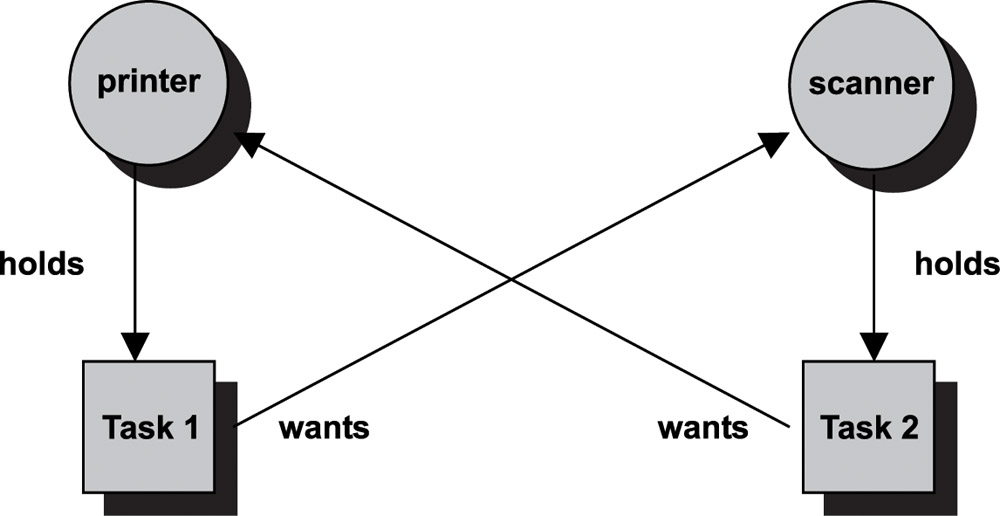
\includegraphics[width=1\textwidth]{figures/deadlock1.jpg}}
	\caption{Gambar Deadlock}
	\label{Gambar}
	\end{figure}
      
      Gambar \ref{Gambar} Contoh gambar pada saat terjadinya deadlock.

\subsection {Masalah Deadlock dan Metode Penanganan Deadlock}
\subsubsection {Masalah Deadlock}
	Deadlock merupakan dampak pengaruh dari sinkronisasi, yaitu dimana satu variabel yang digunakan oleh dua proses yang berbeda. Deadlock selalu tidak terlepas dari yang namanya sumber daya, karena hampir secara keseluruhan merupakan masalah mengenai sebuah sumber daya yang digunakan secara bersamaan. Sebuah Kelompok Proses yang diblok atau diblokir, dimana setiap proses memegang sebuah resource dan kemudian menunggu resource lain dari proses yang berada didalam proses yang sedang diBlok tersebut, biasanya dari semua proses-proses atau resource yang non preemptive..
	
\subsubsection {Metode Penanganan}
	Ada tiga Metode penanganan Deadlock:
	Yang Pertama yaitu, anda harus menggunakan satu protokol yang dapat membuat anda yakin bahwa sistem tersebut tidak akan pernah mengalami kejadian deadlock. Metode ini bisa disebut dengan Deadlock Prevention atau Avoidance.
	
	Yang Kedua, anda harus memberikan izin sistem untuk mengalami kejadian deadlock, namun setelah terjadinya deadlock anda harus dengan cepat segera untuk memperbaiki sistem yang mengalami deadlock tersebut. Metode ini biasanya disebut dengan Deadlock detection and recovery.
	
	Dan yang terakhir, anda hanya mengabaikan semua permasalahan yang terjadi secara bersamaan, dan kemudian menganggap bahwa deadlock tidak akan terjadi, metode ini digunakan dalam berbagai sistem operasi komputer, termasuk windows dan unix.

\begin{table}[H]
\begin{tabular}{|c|c|c|}
\hline
Proses & Jumlah Sumber Daya Digenggam & Maksimum Sumber Daya Dibutuhkan\\
\hline
X   & 2 & 10\\
\hline
Y   & 1 & 3\\
\hline
Z   & 3 & 7\\
\hline
Tersedia 4  &  &\\
\hline
\end{tabular}
\end{table}

\begin{table}[h]
\caption{Kondisi yang menyebabkan Deadlock}
\begin{tabular}{|c|c|}
\hline
Mutual exclusion&Hanya ada satu proses yang boleh memakai sumber daya, dan proses lain yang ingin memakai sumber daya tersebut harus menunggu hingga sumber daya tadi dilepaskan atau tidak ada proses yang memakai sumber daya tersebut.\\
\hline
Hold and wait&Proses yang sedang memakai sumber daya boleh meminta sumber daya lagi maksudnya menunggu hingga benar-benar sumber daya yang diminta tidak dipakai oleh proses lain, hal ini dapat menyebabkan kelaparan sumber daya sebab dapat saja sebuah proses tidak mendapat sumber daya dalam waktu yang lama.\\
\hline
No preemption&Sumber daya yang ada pada sebuah proses tidak boleh diambil begitu saja oleh proses lainnya. Untuk mendapatkan sumber daya tersebut, maka harus dilepaskan terlebih dahulu oleh proses yang memegangnya, selain itu seluruh proses menunggu dan mempersilahkan hanya proses yang memiliki sumber daya yang boleh berjalan. \\
\hline
Circular wait&Kondisi seperti rantai, yaitu sebuah proses membutuhkan sumber daya yang dipegang proses berikutnya.\\
\hline
\end{tabular}
\label{deadlock}
\end{table}

\subsection {Deadlock Detection}
\begin {enumerate}
\item
1. Pendeteksian secara Algoritma, yaitu dengan cara kita mengetahui jika terjadinya deadlock, deadlock terjadi jika suatu permintaan tidak dapat ditangani segera.
	
\item
2. Recovery atau Pemulihan, yaitu yang pertama menggagalkan semua proses deadlock, yang kedua mem backup semua proses yang deadlock dan kemudian silahkan melakukan restart di semua proses yang sedang terjadi, yang ketiga menggagalkan semua proses yang deadlock secara berurutan sehingga tidak akan terjadi lagi deadock, dan yang terakhir yaitu menggagalkan pengalokasian resource secara berurutan hingga tidak ada deadlock.

\end {enumerate}

\subsection {Beberapa hal yang terjadi ketika mendeteksi adanya deadlock}
\begin {enumerate}
\item
1. Permintaan sumber daya dikabulkan selama memungkinkan.
\item
2. Sistem operasi melakukan scanning apakah ada kondisi circular wait secara peiodik.
\item
3. Pemeriksaan dilakukan setiap ada sumber daya yang hendak digunakan.
\item
4. memeriksa dengan algoritma tertentu.
\end {enumerate}

\subsection {Beberapa jalan untuk kembali dari deadlock}
\begin {enumerate}
\item
1. Lewat Preemption, yaitu dengan jauhkan sumber daya dari pemakainya untuk sementara waktu, tujuannya untuk memberikannya pada proses lain. strategi dengan memberikannya kesempatan pada proses lain dengan tanpa diketahui oleh pemilik dari sumber daya itu dan tergantung juga dari sifat sumber daya itu sendiri.
\item
2. Lewat melacak kembali, setelah melakukan prosesn dari preemption tersebut maka secara otomatis proses utama yang diambil sumber dayanya akan stop dan tidak akan melanjutkan prosesnya, oleh karena itu dibutuhkan langkah untuk dapat kembali pada keadaan aman, tetapi untuk menentukan keadaan aman tersebut sangatlah susah.
\item
3. Mematikan proses yang menyebabkan deadlock, ini merupakan cara yang sangat umum digunakan yaitu dengan cara mematikan semua proses yang mengalami deadlock.
\item
4. Menghindari deadlock, pada sistem permintaan untuk sumberdaya biasanya hanya dilakukan sekali saja, sistem harus sudah dapat mengenali bahwa sistem itu aman atau tidak.
\end {enumerate}

\cite{siahaan2015penyelarasan}
\cite{fauzi2013perangkat}
\cite{silberschatz2014operating}


\chapter[Baudrate]
{OS\\ Baud Rate}
%Nama Kelompok: Sistem_Operasi_BaudRate
%Kelas: D4 TI 1B
%Anggota : 
%Kevin Natanael Nainggolan(1174059) 
%Luthfi Muhammad Nabil(1174035)
%Salwaa Tania(1174047)
%Surya Pandu Prananda(1174036)

\section{Baud Rate}

\subsection {Pengertian Baud Rate}
	Baud rate merupakan jumlah terjadi nya suatu perubahan status antara status nol dan status satu dalam waktu satu detik . Contoh nya ialah , suatu saluran memiliki sebuah baud rate 1000 , itu berarti saluran itu mampu mengirimkan setiap detik terjadi 1000 kali perubahan status  .
	
\subsection{Konsep Baud Rate}
Komunikasi secara berturut-turut sudah tidak asing lagi di era teknologi ini, salah satunya dikarenakan jumlah penghantar yang digunakan bisa lebih efektif daripada melakukannya secara sejajar. Mengapa demikian? Karena kata Berturut-turut berarti mengirim satu bit data dan selanjutnya yang diikuti oleh bit-bit data yang lain pada jalur yang sama. Karena itulah kita dapat meringkas penggunaan kabel. Dikarenakan jalur yang dilalui bersamaan, maka kecepatan komunikasi berturut-turut tidak secepat kecepatan komunikasi sejajar. Komunikasi sejajar, dapat mengirim data secara bersamaan melalui beberapa jalur. Namun, untuk proses secara keseluruhan, sistem komunikasi berturut-turut memenuhi berbagai aplikasi microcontroler. Selain itu, sistem komunikasi berturut-turut sering digunakan pada modem, USB, RS-232, dan teman-temannya.Hal yang sangat penting dalam menghubungkan dua perangkat melalui komunikasi berturut-turut adalah memastikan bahwa kedua perangkat berkomunikasi dengan bentuk yang sama, terdapat beberapa parameter yang digunakan untuk membangun komunikasi secara berturut-turut, diantaranya adalah Baud Rate, paket data, parity bit, dan synchronization bit .

Baud rate mengindikasikan seberapa cepat data dikirim melalui komunikasi berturut-turut.Satuan baud rate itu bit per second atau disingkat bps, walaupun untuk kasus tertentu dalam komunikasi sejajar, nilai bps bisa berbeda dengan nilai baud rate. Dugaan saat ini kita berpusat pada komunikasi berturut-turut, dimana setiap detik menyatakan transisi satu bit keadaan. Apabila hal ini terpenuhi, maka nilai baud rate akan sama dengan nilai bit per secondnya. Bit per second ini mengartikan bahwa berapa bit data dapat ditransfer setiap detiknya. Jika kita membalikan nilai bps ini, kita dapat memperoleh keterangan berapa lama waktu yang dipakai saat mengirim 1 bit. Nilai baud rate dapat diatur dengan standar kecepatan, diantaranya 
\begin {itemize}
	\item 1.200bps,
	\item 2.400bps, 
	\item 4.800bps, 
	\item 9.600bps, 
	\item 19.200bps, 
	\item 38.400bps, 
	\item 57.600bps,
	\item 115.200bps. 
\end {itemize}	
	Kecepata yang paling umum digunakan 9.600 bps. Ini adalah nilai yang mana kecepatan komunikasi bukalah suatu hal yang kritis untuk dipertimbangkan. Seperti contoh, jika kita ingin mengetahui nilai dari sensor warna. Mendapatkan data warna dari suatu sensor tidaklah memerlukan kecepatan komunikasi yang terlalu cepat. Agar  error tidak terjadi, kita menggunakan kecepatan standar 9.600 bps.

\begin{figure}[ht]
	\centerline{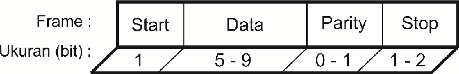
\includegraphics[width=1\textwidth]{figures/serialframe.png}}
	\caption{Serial Frame}
	\label{serialframe}
\end{figure}	
\subsection{Fungsi Baud Rate}
Baud rate dideteksi untuk mengetahui keluaran dari perangkat yang memerlukan basis serial untuk mengecek kecepatan data dan data itu sendiri. \cite{anderson1973method} Secara singkat, mendeteksi baud rate terdiri dari menentukan kecepatan transmisi dari perangkat yang mendapatkan sinyal karena perangkat penerima dapat dengan tepat mendecode sinyal dan mengkonversikannya ke perangkat. Baud rate memberitahu kecepatan data yang dapat dikirim melalui komunikasi serial. Dalam bps sendiri, berarti diketahui berapa kecepatan data yang dialirkan. Biasanya baud rate yang dipakai adalah 9600. Semakin besar baud rate yang dipakai, semakin tinggi kecepatan transfer data. Tetapi makin tinggi kecepatan maka makin beresiko mengalami error data. Untuk itu, disarankan untuk memakai baud rate standar atau dibawah 115.201.

\subsection{ Perbedaan baud rate dengan bit rate }
Kedua nya ini digunakan untuk mengukur kecepatan dalam konektivitas . Baud rate adalah ukuran berapa banyak simbol yang dikirimkan setiap sinyal . Simbol adalah setiap perubahan bentuk gelombang atau pulsa elektrik yang digunakan untuk mentransmisikan data sepanjang medium . Di sisi lain , bitrate adalah ukuran jumlah bit yang ditransmisikan . Dahulu , baud rate dan bit rate di guna kan secara bergantian karena teknik modulasi yang lebih lama dan  hanya memungkin kan satu bit untuk di masuk kan ke dalam setiap simbol . namun sekarang , setiap simbol dapat berisi lebih dari bit , sehingga bitrate menjadi jauh lebih tinggi dari

\subsection{Framing Data}
Framing data adalah teknik penyusunan data untuk dikirim melalui komunikasi serial. Pada gambar \ref{serialframe}, Data yang dikirim melalui komunikasi serial biasanya dari 5 sampai 9 bit. Pada arduino, data yang dipakai berukuran 8 bit. Urutan dari pengiriman data biasanya mengikuti endian tertentu. seperti pengiriman most-significant-bit atau least-significant-bit terlebih dahulu yang dikirim.
\subsubsection{Kit Framing Data}
Start dan Stop bit biasa dikenal sebagai synchronization bit yang biasanya berukuran 2 atau 3 bit. Bit-bit ini mengawali dan mengakhiri pengiriman data. Start bit selalu diberi ukuran 1 bit sedangkan stop bit dapat diberi 1 atau 2 bit tergantung bagaimana pengguna perangkat keras atau pengkonfigurasi perangkat keras menggunakaannya. Jika tidak memerlukan konfigurasi, nilai stop bit dapat dibiarkan menjadi sebesar 1 bit. seperti pada gambar \ref{serialframe}.
Posisi idle pada komunikasi serial bernilai 1. Start bit diidentifikasi dengan adanya transisi dari keadaan idle atau diam. yaitu dari 1 ke 0, sedangkan stop bit adalah kebalikan transisi dari keadaan idle untuk dari 0 ke 1.
Bit Parity dalam framing data bersifat opsional dan dapat diabaikan. Parity bit digunakan untuk transfer data yang dipengaruhi oleh noise. Namun penggunaan bit parity dapat memperlambat kecepatan komunikasi atau transfer. Penggunaan bit parity juga dibutuhkan sebuah sinkronisasi antara transmitter dengan receiver karena dilakukan untuk mengurangi kemungkinan kesalah dalam interpretasi data dalam perangkat keras.

\subsection{Contoh Pengiriman Data}
Dengan contoh saat kita mau mengirim kata OK. komunikasi akan memiliki 2 paket data. Kode ASCII untuk ;O' adalah 79 dalam desimal sedangkan huruf 'K' adalah 75. Data yang terkirim lebih dahulu adalah least-significant bit. Karena data dikirim dengan kecepatan 9600 bps, maka setiap bit memerlukan waktu selama 1/9600 = 104 mikrodetik/bit. Dalam arduino, setting baud rate dapat dilakukan dengan kode :
\begin{verbatim}
Serial.begin(9600);
\end{verbatim}
Kode tersebut menandakan bahwa kecepatan serial adalah 9600 bps atau 9600 bit per detik.



\chapter[PySerial]
{OS\\ PySerial}
\section{Py Serial}

	\subsection{Python}
	Python adalah bahasa pemrograman yang dibuat oleh Guido van Rossum dan populer sebagai bahasa pemrograman scripting dan Web. Mengacu pada ide wikipedia, Python adalah bahasa pemrograman interpretatif multiguna dengan filosofi desain yang berfokus pada keterbacaan kode. 
	Python dikenal sebagai bahasa pemrograman yang menggabungkan nilai nilai kapabilitas, kemampuan, dengan sintaks kode yang sangat begitu jelas, dan dilengkapi dengan fungsi penyimpanan standar yang menjadikannya komprehensif dan komprehensif. 
	Python mendukung pemrograman multi-paradigma, khususnya, tetapi tidak terbatas, pada pemrograman berorientasi objek, pemrograman imperatif, dan pemrograman fungsional. 
	Python memiliki salah satu fitur yang sangat unik yaitu sebagai bahasa pemrograman dinamis yaitu yang datang dengan manajemen memori otomatis. Seperti bahasa 
	pemrograman dinamis lainnya, python umumnya digunakan sebagai bahasa scripting meskipun dalam prakteknya penggunaan bahasa ini lebih luas termasuk konteks penggunaan yang umumnya tidak dilakukan menggunakan bahasa scripting. 
	Python dapat digunakan untuk berbagai tujuan pembuatan perangkat lunak atau pun pengembangan perangkat lunak dan dapat dijalankan di berbagai platform sistem operasi. Python adalah salah satu contoh bahasa tingkat tinggi. 
	Contoh lain dari bahasa high-rise adalah pascal, c ++, perl, java, dan seterusnya. Sedangkan bahasa tingkat rendah adalah bahasa mesin atau bahasa assembly. 
	Secara sederhana. komputer hanya dapat menjalankan program yang ditulis dalam bahasa mesin. Karena itu. jika sebuah program ditulis dalam bahasa tinght yang tinggi. maka program tersebut harus diolah terlebih dahulu sebelum dapat dijalanlon di komputer. 
	Ini adalah salah satu kekurangan bahasa tingkat tinggi yang membutuhkan waktu untuk memproses suatu program sebelum dijalankan. Namun, bahasa tingkat tinggi memiliki banyak kelebihan. Bahasa tinglrat yang tinggi mudah dipelajari. mudah ditulis. mudah dibaca. dan tentu saja mudah menemukan kesalahan. Bahasa tingkat tinggi juga mudah dibawa untuk dicocokkan dengan mesin yang menjalankannya. 
	
	\subsection{Kelebihan}
		\begin{itemize}
			\item Dapat lebih cepat dalam pembuatan sistem aplikasi.
			\item Programnya lebih fleksible, singkat, dan sederhana.
			\item Dapat lebih mudah hindari pencatatan kode.
			\item Dapat lebih cepat dalam membuat sistem aplikasi dengan menggunakan objek yang telah ada.
			\item Mempunyai dukungan pemrograman dengan skala yang besar.
			\item Ekstensinya lebih sederhana juga berkas binernya kecil.
			\item Dapat memodifikasi atau merubah aplikasi tanpa menghentikannya.
			\item Kecepatan dalam mengeksekusi bertambah juga melindungi kode sumber.
		\end{itemize}
		
	\subsection{Kekurangan}
		\begin{itemize}
			\item Pyhton tidak efisien sebagai sebuah statis, berbeda dengan bahasa C yang dapat mempunyai penugasan yang lebih luas dari python.
			\item Python adalah sebuah interpreter, jadi tidak begitu baik dalam pengantar komponen performa kritis.
			\item Tidak bisa menjadi dasar bahasa pemrograman implementasi di beberapa komponen.
			\item Tidak memberikan keefensiensian yang menyeluruh.
		\end{itemize}
		
	\subsection{Komunikasi Serial}
		Langkah - langkah untuk melakuan komunikasi serial adalah sebagai berikut :
		
		\begin{enumerate}
			\item Open Phyton Shell
			
				\begin{figure}[ht]
			\centerline{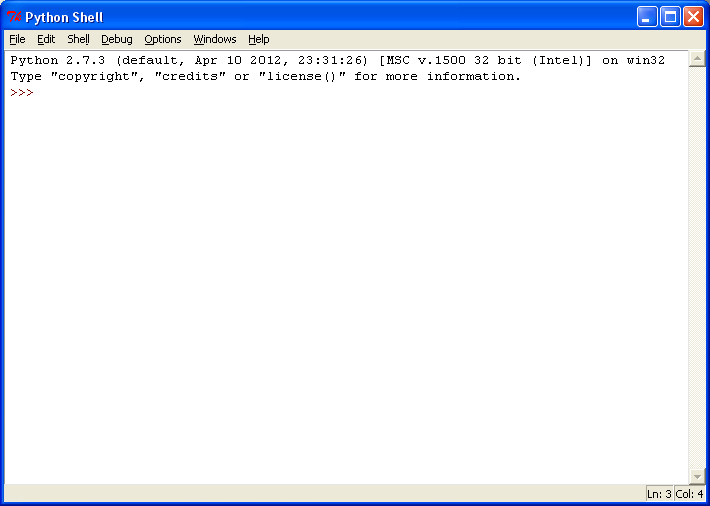
\includegraphics[width=0.5\textwidth]{figures/pyshell.png}}
			\caption{Python Shell}
			\label{pyshell}
			\end{figure}
			
			\item Buat new window seperti atau bisa juga dengan (Ctrl + N), agar muncul window baru.
				
				\begin{figure}[ht]
			\centerline{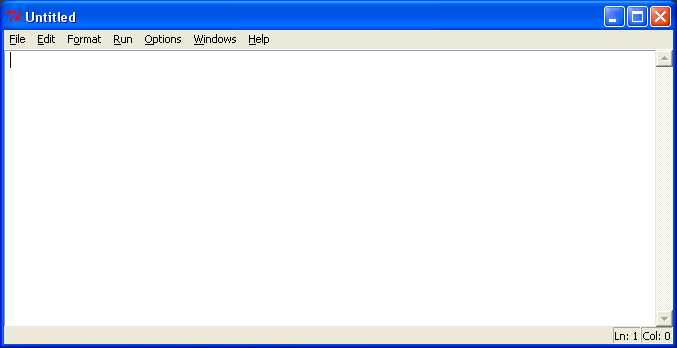
\includegraphics[width=0.5\textwidth]{figures/pyshellnew.png}}
			\caption{New Window}
			\label{pyshellnew}
			\end{figure}
			
			\item Copykan atau ketikkan script ini :
				\begin{verbatim}
					    import serial
						ser = serial.Serial(‘com10’,9600,timeout=1)
						from Tkinter import *
						root=Tk()
						def task():
						a=ser.readline(1)
						print “nilai= ” + a
						root.after(200,task)
						root.after(200,task)
						root.mainloop()
					\end{verbatim}
					
			\item Dibawah ini adalah hasilnya :
			akan muncul window:
			
			\begin{figure}[ht]
			\centerline{
\includegraphics[width=0.5\textwidth]{figures/tkser.png}}
			\caption{TK Window}
			\label{tkser}
			\end{figure}
			
			dan di Python Shell akan muncul :
			
			\begin{figure}[ht]
			\centerline{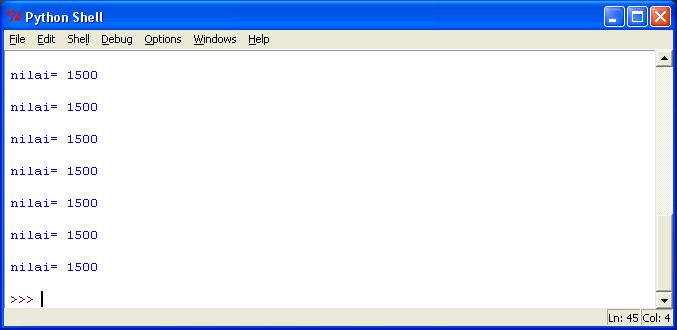
\includegraphics[width=0.5\textwidth]{figures/tkpython.png}}
			\caption{TK Window}
			\label{tkpython}
			\end{figure}
			
		\end{enumerate}
		
		Penjelasannya : 
		\begin{itemize}
			\item import serial
			bagian diatas ini mempunyai fungsi untuk melibatkan module serial sehingga dapat digunakan pada Python.
			
			\item \begin{verbatim} ser = serial.Serial(‘com10’,9600,timeout=1)\end{verbatim}
			Bagian diatas ini berfungsi sebagai pendeklerasian variabel ser sebagai serial port yang propertinya adalah konfigurasi nomer port= COM10, baudrate= 9600, dan timeout=1.
			\item \begin{verbatim} a=ser.readline() \end{verbatim}
			Bagian diatas ini berfungsi untuk membaca data dari serial lalu menampungnya pada variabel a sebagai buffer.
			\item \begin{verbatim} print “nilai= ” + a \end{verbatim} 
			Bagian diatas ini berfungsi untuk tampilkan nilai yang didapat di Python Shell. 
			\item \begin{verbatim} root.after(200,task) \end{verbatim}
			Bagia di atas ini berfungsi untuk melakukan suatu schedule setiap 200 milidetik.
			\item \begin{verbatim} root.after(200,task)	\end{verbatim}
			Bagian diatas ini berfungsi untuk mengulang suatu schedule setiap 200 milidetik.
			\item \begin{verbatim} root.mainloop() \end{verbatim}
			Bagian diatas ini berfungsi untuk melakukan perulangan atau loop.
		\end{itemize}
	
	\cite{nurjanahhack}
	\cite{rossum1995python}


\chapter[Serial Communication di Linux]
{OS\\ Serial Comm}
%kelompok 1 Sistem Operasi (Semaphore)
%Kelas D4 TI 1B
%Adam Noer Hidayatullah 1174097
%Ichsan Hizman
%Teddy
%Nisrina Aulia
%Irvan Rizkiansyah 1174043

\section{Komunikasi Serial pada Linux}
	
	\subsection{Konsep Dasar Komunikasi Serial}
	Suatu komunikasi yang dilakukan dimana suatu pengiriman data dilakukan per bit ialah dinamakan komunikasi serial, sehingga akan lebih lambat jika dibandingkan dengan komunikasi parallel seperti yang ada pada port printer yang dapat mengirim 8 bit sekaligus dalam sekali detak.
	Terdapat 2 macam cara komunikasi data serial yaitu :
		\begin{enumerate}
			\item Komunikasi data serial sinkron
			\item Komunikasi data serial asinkron
		\end{enumerate}
	
	Terdapat 2 kelompok device pada komunikasi serial yaitu :
		\begin{enumerate}
			\item Data Communication Equipment (DCE)
			Contohnya seperti scanner, printer, modem dan yang lainnya.
			\item Data Terminal Equipment (DTE)
			Contohnya sepertia terminal yang ada pada komputer.
		\end{enumerate}
	
	Keuntungan menggunakan port serial
		\begin{itemize}
			\item Masalah cable loss tidak akan menjadi suatu masalah yang besar pada komunikasi dengan kabel yang panjang, dari pada menggunakan kabel paralel. Port paralel akan mentransmisikan 0 pada tegangan 0 volt dan 1 di tegangan 1 volt, sedangkan port serial akan mentransmisikan 1 di tegangan -3 - -25 volt dan 0 di tegangan +3 - +25 volt.
			\item Hanya membutuhkan jumlah kabel yang sedikit, menggunakan 3 kabel saja pun bisa yaitu saluran Ground, saluran Transmit Data, saluran Receive Data.
			\item Populernya penggunaan mikrokontroler dan kebanyakan mikrokontroler dilengkapi dengan Serial Communication Interface (SCI) yang bisa dipaki untuk melakukan komunikasi dengan port serial pada komputer.
		\end{itemize}

	\subsection{Interprocess Communication}
	komunikasi antar proses untuk mengirim data dari satu proses ke proses yang lain, baik antar proses dalam satu komputer maupun proses dalam komputer yang berbeda
	karakteristik dari Interprocess Communincation yaitu:
		\begin{enumerate}
			\item komunikasi Synchronous dan asynchronous
				pada Sinkronisasi Synchronous, proses pengiriman dan penerimaan pada setiap pesan dan sistem ini akan berfungsi, jika sistem mengirim pesan, maka sistem hanya akan dapat merespon, sampai pesan selesai. Dalam komunikasi asynchronous, komunikasi ini dapat langsung memproses pesan, begitu pesan berada di buffer lokal, dan mengirim pesan dengan benar.
			\item Message destinations
					tempat tujuan dari sebuah pesan yang terdapat pada  sebuah computer adalah local port, yang didefinisikan berarti sebagai variable angka dengan tipe integer. Sebuah port pasti mempunyai satu penerima, akan tetapi bisa memiliki banyak pengirim.
			\item Reliability
					Keandalan suatu sistem dapat dilihat dari validitas dan integritas sistem.
					Sistem bila dilihat dari validitas, dapat dikatakan handal jika pesan yang disampaikan dijamin hingga tidak ada pesan yang hilang atau jatuh, dan sebaliknya.
			\item Ordering
				  menginginkan pesan yang terkirim dari pengirim dapat diterima sesuai dengan urutan grouping / ordering berdasarkan pesan awal yang terikirim.
		\end{enumerate}

		
	\subsection{Koneksi Linux ke Serial Port}
	Untuk melakukan setting pada suatu perangkat, terkadang harus masuk terlebuh dahulu ke dalam console box. Biasanya akan menggunakan hyperterminal, namun software bawaan seperti itu tidak terdapat pada linux pada saat linux terinstall. Maka dari itu terdapat sebuah software yang dapat digunakan pada linux untuk melakukan komunikasi serial yaitu minicom untuk menggantikan hyperterminal.
	
	Software terminal minicom dapat di install dengan mudah di linux. Pertama buka terminal pada linux lalu ketik perintah :

	sudo apt-get install minicom

	Setelah itu software akan terinstall. Kemudian koneksikan ke perangkat yang akan digunakan menggunakan kabel console pada port serial. Lalu cek pada terminal linux dengan menggunakan perintah :

	dmesg | grep tty
	
	Perintah tersebut berguna untuk mengetahui port mana saja yang digunakan, seperti pada gambar dibawah ini
	
	\begin{figure} [ht]
	\centerline{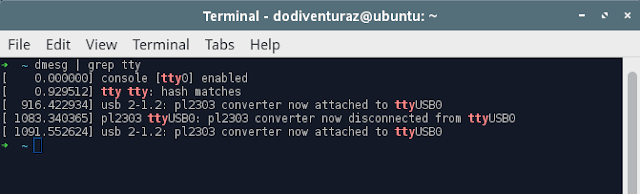
\includegraphics[width=1\textwidth]{figures/serialunix.png}}
	\caption{Gambar Status Serial}
	\label{statusserial}
	\end{figure}
	
	\ref{serialunix}
	
	Lalu ketikkan perintah :
	
	sudo minicom -s
	
	dan akan muncul seperti dibawah ini :
	
	\begin{table}[H]
		\begin{tabular}{|c|}
			\hline
			----configuration----\\
			\hline
			Filenames and paths\\
			\hline
			File transfer protocols\\
			\hline
			Serial port setup\\
			\hline
			Modem and dialing\\
			\hline
			Screen and keyboard\\
			\hline
			Save setup as dfl\\
			\hline
			Save setup as..\\
			\hline
			Exit\\
			\hline
			Exit from Minicom\\
		\end{tabular}
	\end{table}
	
	Kemudian pilih Serial Port Setup untuk mengetahui port yang terdeteksi, lalu akan muncul tampilan sebagai berikut :
	
	\begin{figure} [ht]
	\centerline{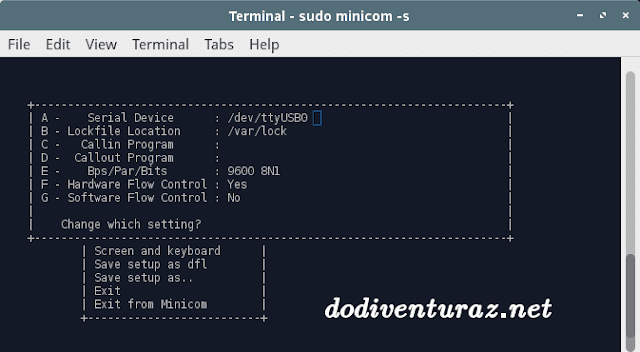
\includegraphics[width=1\textwidth]{figures/minicom.png}}
	\caption{Gambar minicom}
	\label{minicom}
	\end{figure}
	
	\ref{minicom}
	
	Lalu lakukan konfigurasi yang diperlukan sesuai kebutuhan yang diperlukan. Setelah konfigurasi selesai kembali ke menu utama dan pilih Save Setup as dfl. Kemudian pilih Exit, dan akan kembali ke terminal linux sebelumnya, kemudian ketikan perintah 
	
	minicom
	Maka Perangkat akan terkoneksi sesuai keinginan.

	




\chapter[SERIALCOMWINDOWS]
{OS\\ SERIALCOMWINDOWS}
\section{Serial Com Windows}
	\subsection{Membuka Port}
		\begin{enumerate} 
			Dokumentasi SDK Platform menyatakan bahwa ketika membuka port komunikasi, panggilan ke CreateFile memiliki persyaratan berikut:
				\item 1. fdwShareMode harus nol. Port komunikasi tidak dapat dibagikan dengan cara yang sama seperti file yang dibagikan. Aplikasi yang menggunakan TAPI dapat menggunakan fungsi TAPI untuk memfasilitasi berbagi sumber daya antar aplikasi. Untuk aplikasi yang tidak menggunakan TAPI, penanganan warisan atau duplikasi diperlukan untuk berbagi port komunikasi. Berurusan dengan duplikat berada di luar cakupan artikel ini; silakan merujuk ke dokumentasi Platform SDK untuk informasi lebih lanjut.
				\item 2. fdwCreate harus menentukan bendera OPEN_EXISTING.
				\item 3. hTemplateFile parameter harus NULL.
			Satu hal yang perlu diperhatikan tentang nama port adalah bahwa mereka secara tradisional telah COM1, COM2, COM3, atau COM4. Windows API tidak menyediakan mekanisme apa pun untuk menentukan port apa yang ada pada sistem. Beberapa sistem bahkan memiliki lebih banyak port daripada maksimum tradisional empat. Vendor perangkat keras dan pembuat perangkat serial-driver bebas memberi nama port apa pun yang mereka sukai. Untuk alasan ini, yang terbaik adalah pengguna memiliki kemampuan untuk menentukan nama port yang ingin mereka gunakan. Jika port tidak ada, kesalahan akan terjadi (ERROR_FILE_NOT_FOUND) setelah mencoba membuka port, dan pengguna harus diberitahu bahwa port tidak tersedia.
		\end{enumerate}
		\begin{enumerate}
		I / O tumpang tindih
				/ O yang tumpang tindih tidak sesederhana I / O non-tumpang tindih, tetapi memungkinkan lebih banyak fleksibilitas dan efisiensi. Sebuah port terbuka untuk operasi tumpang tindih memungkinkan beberapa utas untuk melakukan operasi I / O pada saat yang bersamaan dan melakukan pekerjaan lain ketika operasi sedang menunggu. Lebih jauh lagi, perilaku operasi yang tumpang tindih memungkinkan satu utas untuk mengeluarkan banyak permintaan yang berbeda dan bekerja di latar belakang sementara operasi masih menunggu.

				Baik dalam aplikasi single-threaded maupun multithread, beberapa sinkronisasi harus dilakukan antara mengeluarkan permintaan dan memproses hasilnya. Satu utas harus diblokir sampai hasil operasi tersedia. Keuntungannya adalah I / O yang tumpang tindih memungkinkan utas untuk melakukan beberapa pekerjaan antara waktu permintaan dan penyelesaiannya. Jika tidak ada pekerjaan yang dapat dilakukan, maka satu-satunya kasus untuk I / O yang tumpang tindih adalah memungkinkan untuk respon pengguna yang lebih baik.

		\end{enumerate}

	\begin{figure}[ht]
		\centerline{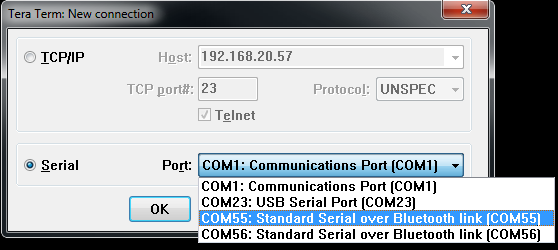
\includegraphics[width=1\textwidth]{figures/seria.png}}
		\caption{Serial Com Windows}
		\label{seria}
	\end{figure}
	Gambar \ref{seria} Contoh gambar.
		\begin{verbatim}
			HANDLE hComm;
			hComm = CreateFile( gszPort,  
                    GENERIC_READ | GENERIC_WRITE, 
                    0, 
                    0, 
                    OPEN_EXISTING,
                    FILE_FLAG_OVERLAPPED,
                    0);
			if (hComm == INVALID_HANDLE_VALUE)
				// error opening port; abort
		\end{verbatim}
	\subsection{Membaca dan menulis}
		\begin{enumerate}
			\item Membaca dari dan menulis ke port komunikasi di Windows sangat mirip dengan file input / output (I / O) di Windows. Bahkan, fungsi yang melengkapi I / O file adalah fungsi yang sama yang digunakan untuk serial I / O. I / O dapat dilakukan dengan salah satu dari dua cara: tumpang tindih atau tidak tumpang tindih. Dokumentasi SDK Platform menggunakan istilah asinkron dan sinkron untuk mengkonotasikan jenis operasi I / O ini. Artikel ini, bagaimanapun, menggunakan istilah yang tumpang tindih dan tidak terabaikan.
			\item Nonoverlapped I / O akrab bagi kebanyakan pengembang karena ini adalah bentuk tradisional I / O, di mana operasi diminta dan diasumsikan lengkap ketika fungsi kembali. Dalam kasus I / O yang tumpang tindih, sistem dapat kembali ke pemanggil segera bahkan ketika operasi tidak selesai dan akan memberi sinyal kepada pemanggil ketika operasi selesai. Program ini dapat menggunakan waktu antara permintaan I / O dan penyelesaiannya untuk melakukan beberapa pekerjaan latar belakang.
				\subsubsection{Bacaan}
					\begin{enumerate}
						\item Fungsi ReadFile menerbitkan operasi baca. ReadFileEx juga mengeluarkan operasi baca, tetapi karena tidak tersedia pada Windows 95, itu tidak tercakup dalam artikel ini. Berikut adalah potongan kode yang merinci cara mempublikasikan permintaan baca. Perhatikan bahwa fungsi memanggil fungsi untuk memproses data jika ReadFile mengembalikan TRUE. Ini adalah fungsi yang sama yang disebut jika operasi menjadi tumpang tindih. Perhatikan flag fWaitingOnRead yang didefinisikan oleh kode; ini menunjukkan apakah operasi baca tumpang tindih atau tidak. Ini digunakan untuk mencegah penciptaan operasi baca baru jika mereka luar biasa.
				
				\begin{verbatim}
				\item DWORD dwRead;
					BOOL fWaitingOnRead = FALSE;
					OVERLAPPED osReader = {0};

						// Create the overlapped event. Must be closed before exiting
						// to avoid a handle leak.
						osReader.hEvent = CreateEvent(NULL, TRUE, FALSE, NULL);

						if (osReader.hEvent == NULL)
						// Error creating overlapped event; abort.

						if (!fWaitingOnRead) {
						// Issue read operation.
						if (!ReadFile(hComm, lpBuf, READ_BUF_SIZE, &dwRead, &osReader)) {
						if (GetLastError() != ERROR_IO_PENDING)     // read not delayed?
						// Error in communications; report it.
					else
						fWaitingOnRead = TRUE;
				}
					else {    
						// read completed immediately
						HandleASuccessfulRead(lpBuf, dwRead);
			}
		}
				\end{verbatim}

				\begin{enumerate}
						\item Bagian kedua dari operasi yang tumpang tindih adalah deteksi penyelesaiannya. Pegangan acara dalam struktur OVERLAPPED diteruskan ke fungsi WaitForSingleObject, yang akan menunggu hingga objek diberi isyarat. Setelah acara ditandai, operasi selesai. Ini tidak berarti bahwa itu berhasil diselesaikan, hanya saja itu selesai. Fungsi GetOverlappedResult melaporkan hasil operasi. Jika kesalahan terjadi, GetOverlappedResult mengembalikan FALSE dan GetLastError mengembalikan kode kesalahan. Jika operasi selesai dengan sukses, GetOverlappedResult akan mengembalikan TRUE.

						
						Catatan GetOverlappedResult dapat mendeteksi penyelesaian operasi, serta mengembalikan status kegagalan operasi. GetOverlappedResult mengembalikan FALSE dan GetLastError mengembalikan ERROR_IO_INCOMPLETE ketika operasi tidak selesai. Selain itu, GetOverlappedResult dapat dibuat untuk memblokir hingga operasi selesai. Ini secara efektif mengubah operasi yang tumpang tindih menjadi operasi non-tumpang tindih dan dicapai dengan melewatkan TRUE sebagai parameter bWait.
				\end{enumerate}


			
		\end{enumerate}
			\subsubsection{Penulisan}
				\begin{enumerate}
					\item Pengarsipan data dari port komunikasi sangat mirip dengan membaca, karena menggunakan banyak API yang sama. Cuplikan kode di bawah ini menunjukkan cara menghapus dan menunggu operasi tulis selesai.
				\end{enumerate}
				\begin{verbatim}
				BOOL WriteABuffer(char * lpBuf, DWORD dwToWrite)
{
   OVERLAPPED osWrite = {0};
   DWORD dwWritten;
   DWORD dwRes;
   BOOL fRes;

   // Create this write operation's OVERLAPPED structure's hEvent.
   osWrite.hEvent = CreateEvent(NULL, TRUE, FALSE, NULL);
   if (osWrite.hEvent == NULL)
      // error creating overlapped event handle
      return FALSE;

   // Issue write.
   if (!WriteFile(hComm, lpBuf, dwToWrite, &dwWritten, &osWrite)) {
      if (GetLastError() != ERROR_IO_PENDING) { 
         // WriteFile failed, but isn't delayed. Report error and abort.
         fRes = FALSE;
      }
      else
         // Write is pending.
         dwRes = WaitForSingleObject(osWrite.hEvent, INFINITE);
         switch(dwRes)
         {
            // OVERLAPPED structure's event has been signaled. 
            case WAIT_OBJECT_0:
                 if (!GetOverlappedResult(hComm, &osWrite, &dwWritten, FALSE))
                       fRes = FALSE;
                 else
                  // Write operation completed successfully.
                  fRes = TRUE;
                 break;
            
            default:
                 // An error has occurred in WaitForSingleObject.
                 // This usually indicates a problem with the
                // OVERLAPPED structure's event handle.
                 fRes = FALSE;
                 break;
         }
      }
   }
   else
      // WriteFile completed immediately.
      fRes = TRUE;

   CloseHandle(osWrite.hEvent);
   return fRes;
}
\end{verbatim}	

\subsection{Serial Status}
	\begin{enumerate}
		\item Ada dua metode untuk mengambil status port komunikasi. Yang pertama adalah dengan mengatur event mask yang menyebabkan pemberitahuan aplikasi ketika peristiwa yang diinginkan terjadi. Fungsi SetCommMask mengatur masker kejadian ini, dan fungsi WaitCommEvent menunggu kejadian yang diinginkan terjadi. Metode kedua untuk mengambil status port komunikasi adalah secara berkala memanggil beberapa fungsi status yang berbeda. Polling, tentu saja, tidak efisien dan tidak direkomendasikan. Berikut ini contoh fungsi SetCommMask:
	\end{enumerate}
	\begin{verbatim}
	DWORD dwStoredFlags;

dwStoredFlags = EV_BREAK | EV_CTS   | EV_DSR | EV_ERR | EV_RING |\
                EV_RLSD | EV_RXCHAR | EV_RXFLAG | EV_TXEMPTY ;
if (!SetCommMask(hComm, dwStoredFlags))
   // error setting communications mask
\end{verbatim}

\cite{bai2004windows}
\cite{carvey2005tracking}
\cite{boling2003programming}			


\chapter[usb to serial]
{OS\\ usb to serial}
%Nama Kelompok: Sistem_Operasi_Deadlock
%Kelas: D4 TI 1B
%Alit Fajar Kurniawan(1174057) 
%Muhammad Iqbal Panggabean(1174063)
%Muhammad Afra Faris(1174041)
%Khadijah Hasanah Puteri Harahap(1174044)

\section {USB TO SERIAL}

\subsection {Pengertian USB}
\subsubsection {Apa itu USB ?}
	Universal Serial Bus atau yang disingkat dengan USB adalah sebuah teknologi yang dapat memungkinkan para penggunanya untuk dapat menghubungkan hardware eksternal contohnya seperti printer, keyboard, harddisk, flashdisk dan perangkat keras lainnya. kecepatan trnasfer data yang didukung oleh USB sebesar 12 Mbps. pada saat ini semua PC sudah memiliki port USB sendiri minimal 2 buah port USB.

\subsection {Jenis-jenis usb}
\begin {enumerate}
\item
	USB 1.1 : Versi kabel USB 1.1 adalah versi yang pertama yang dirilis sekitar Agustus 1998 dan mulai banyak digunakan di berbagai perangkat elektronik. Versi original-nya, USB 1.0 tidak pernah digunakan pada perangkat elektronik. Versi kabel USB 1.1 ini Memiliki kecepatan up to 12 Mbps. logo yang di punyai oleh USB 1.1 ini berwarna biru dan simbol berbentuk trisula. Namun sekarang , Versi kabel USB ini sudah tidak digunakan lagi.
\item
	USB 2.0 : versi kabel USB 2.0 adalah versi yang kedua yang di rilis pada tahun 2000. Kabel usb ini memiliki kecepatan maximum up to 480Mbps dengan Hi-Speed mode atau pada Full-Speed mode memiliki kecepatan 12 Mbps . Kabel USB ini memiliki supply tegangan maximumnya ( max power out put ) adalah 2.5V, 1.8A dan akan tetap berfungsi baik jika dihubungkan dengan versi sebelumnya ( backward - compatible with USB 1.1 )
	
	Kabel USB 2.0 ini memiliki logo berwarna biru dengan tambahan tulisan HI-SPEED di atasnya dengan dasar merah. Simbol seperti trisula dengan tambahan tanda “ + ” di atasnya. Terkadang , hanya berupa sebuah trisula saja untuk menunjukkan USB yang digunakan adalah USB 2.0 , karena USB 1.1 sudah tidak digunakan lagi. Namun fungsinya kabel usb ini masih sama dengan versi sebelumnya.
\item
	USB 3.0 : Versi kabel USB 3.0 adalah versi yang ketiga yang rilis pada tahun 2008 . Kabel USB 2.0 ini memiliki kecepatan up to 5 Gbps dalam mode SuperSpeed. pada umumnya pada versi kabel USB 3.0 memiliki konektor dan soket USB berwarna biru . Maksudnya ialah sebagai tanda untuk membedakan USB 3.0 dengan versi sebelumnya .
	
	Versi kabel USB 3.0 dikenal sebagai USB Super Speed dengan gambar logo bertuliskan SUPERSPEED. Kabel USB 3.0 ini , memiliki simbol yang berbeda dengan versi kabel USB yang sebelumnya. Perbedaannya adalah ada tambahan huruf SS di pangkal trisula. USB 3.0 memiliki tampilan yang sama seperti USB 2.0 sehingga cukup kompatibel dengan USB 2.0.
	
\item
	USB 3.1 : Versi kabel USB 3.1 adalah versi yang keempat yang rilis pada tahun 2013. Kabel USB 3.1 ini memiliki kecepatan 2 kali lebih tinggi dari versi USB 3.0 yaitu 10 Gbps. Versi USB 3.1 ini juga dikenal dengan sebutan USB Super Speed + atau Super Speed USB 10 Gbps atau standar dengan Thunderbolt ( milik Apple ) . Versi USB 3.1 ini sangat kompatibel dengan USB 3.0 dan USB 2.0 . USB 3.1 ini memiliki tiga power supply tegangan , yaitu 2A pada tegangan 5V (tegangan max 10W), 5A pada tegangan 12V ( tegangan max 60W), dan 5A pada tegangan 20V ( egangan max 100W ) .
\end {enumerate}
	
\subsection {Ada Beberapa Keistimewaan dari USB}
\begin {enumerate}
\item
 PC atau komputer dapat dijadikan sebagai sebuah host
\item
 127 perangkat atu lebih dapat terhubung ke PC atau komputer dengan menggunkan hub USb secara langsung
\item
 Jika menggunakan kabel USB secara langsung hanya bisa mencapai 5 meter dan apabila menggunakan perangkat hub dapat sampai 30 meter jangkauannya
\item
 Sifat perangkat USB 'hot swappable' yang artinya apabila ada perangkat keras yang telah menggunakan port USB sifatnya plug and play
\end {enumerate}	

\subsection {Cara menghubungkan USB flash disk dengan komputer}
	USB port digunakan oleh flash disk denga tujuan untuk dapat mnghubungkan dengan komputer. fungsi dari flash disk itu sendiri yaitu untuk dapat menyimpan data dan flash disk juga memiliki batas maksimal penyimpanan. Mempelajari tentang bagaimana cara menghubungkan flash disk dengan komputer merupakan hal yang sangat mudah karena kita hanya memasukkan flash disk kedalam port USB yang tersedia di PC atau komputer. Ini merupakan salah satu cara komunikasi antara komputer atau PC dengan hardware yng dihubungkan dengan komputer atau PC dan dilakukan melalui USB To Serial.
	
	\begin{figure}[ht]
	\centerline{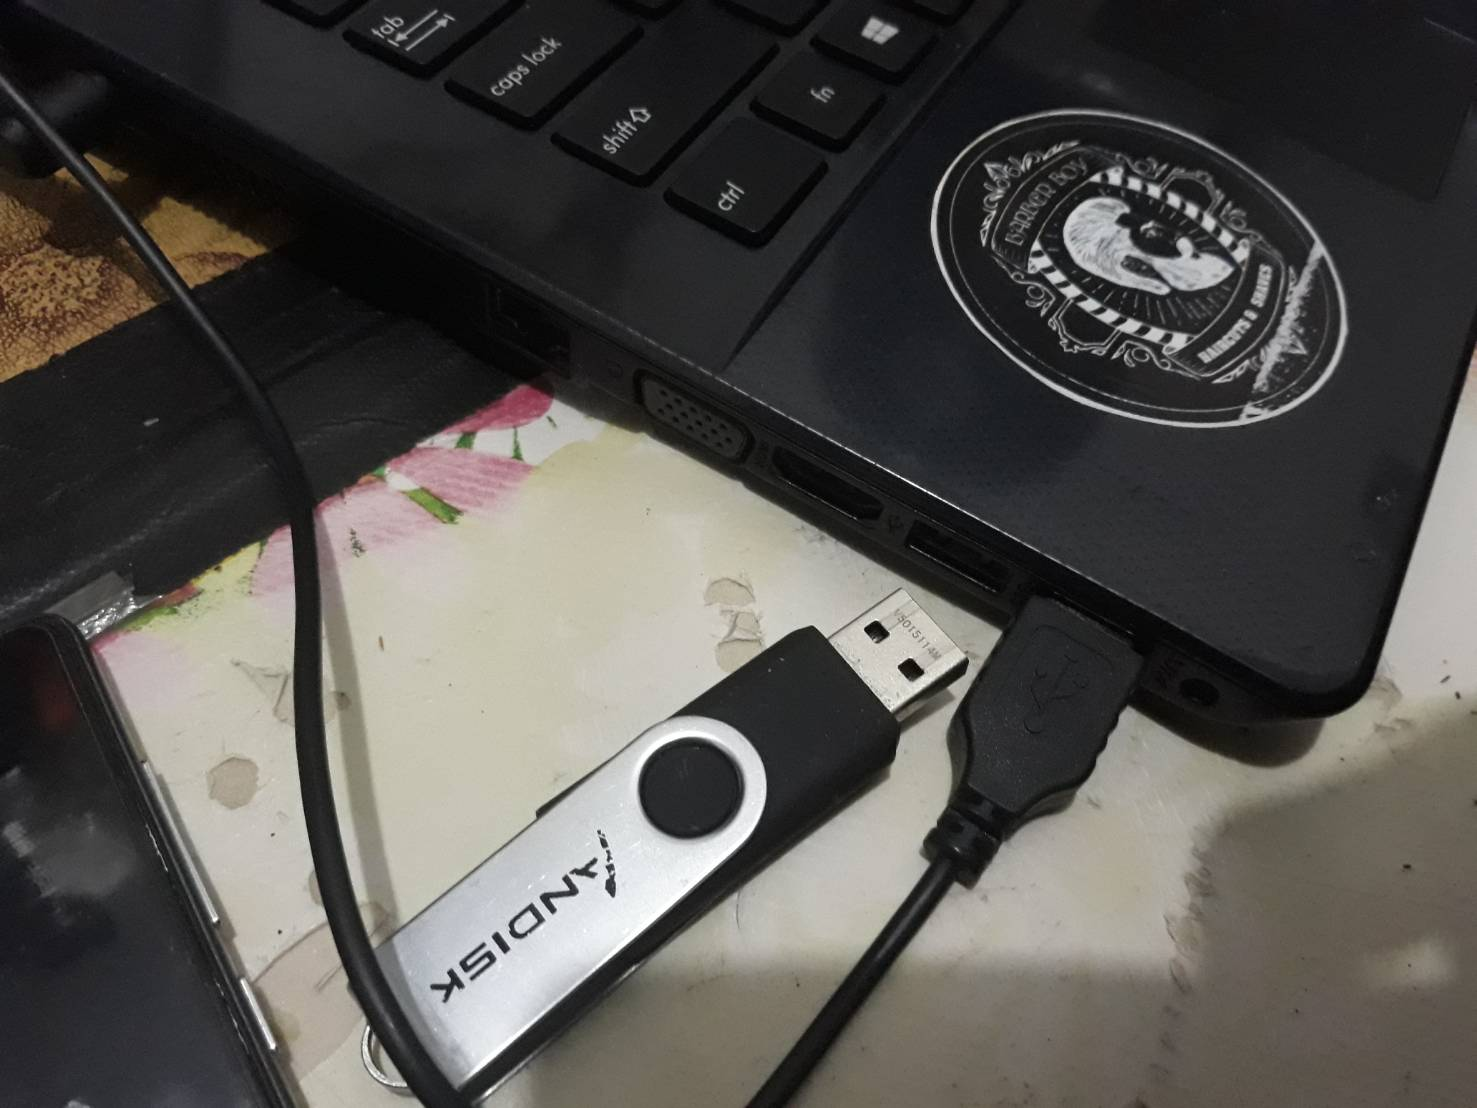
\includegraphics[width=1\textwidth]{figures/usb1.jpg}}
	\caption{Gambar memasukkan flash disk kedalam port usb pada PC}
	\label{Gambar}
	\end{figure}
      
      Gambar \ref{Gambar} Contoh gambar memasukkan flash disk kedalam port usb pada PC.
	  
\subsection {Beberapa istilah}	  
\begin{table}[H]
\begin{tabular}{|c|c|c|c|c|}
hline
No & Istilah & Arti dari Istilah\\
\hline
1   & Peripheral & Perangkat\\
2   & Hub & Sebuah alat yang digunakan untuk menghubungkan dan memperkuat sinyal dari satu PC dengan PC yang lain\\
3   & Plug and Play & Dapat langsung dikethui dan bisa digunakan oleh PC\\
4   & Port & Tempat untuk memasukkan USB\\
\hline
\end{tabular}
\end{table}


\subsection {Proses yang terjadi di USB}
	Ketika USB dimasukkan kedalam port USB pada komputer atau PC maka komputer atau PC akan mendata perangkat yang sudah tersambung ke port USB dan kemudian dilakukannya persiapan lamat memori kepada setiap perangkat yang terpasang. Proses ini disebut dengan enumerasi.
	
	
	\begin{figure}[ht]
	\centerline{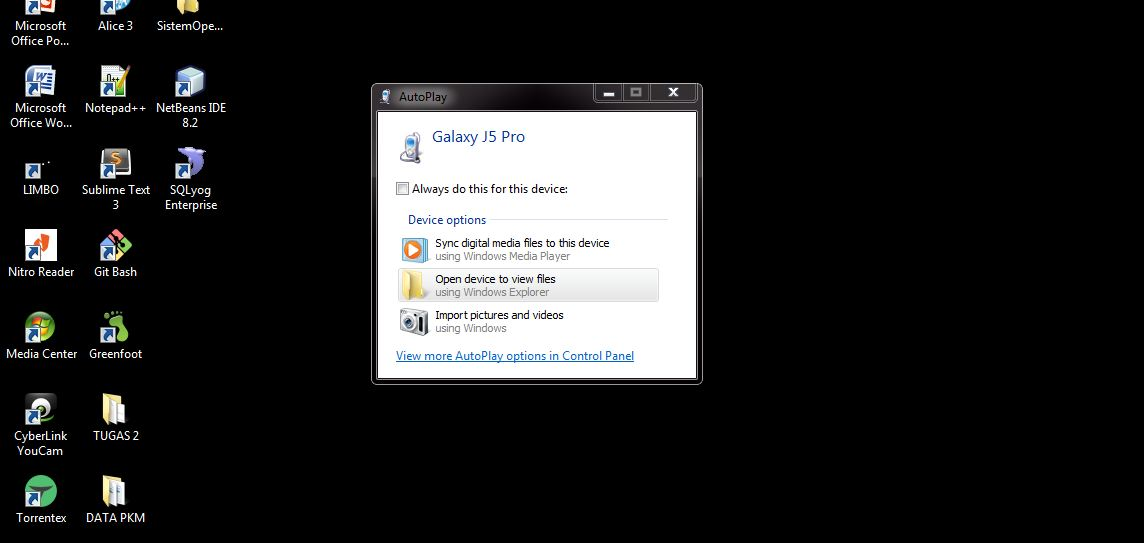
\includegraphics[width=1\textwidth]{figures/usb2.jpg}}
	\caption{Gambar proses enumerasi}
	\label{Gambar}
	\end{figure}
      
      Gambar \ref{Gambar} Contoh gambar proses enumerasi.
      
      	\cite{kulyukin2004rfid}
	\cite{turang2015pengembangan}



%\chapter[DeadLock]
%{OS\\ DeadLock}
%%Nama Kelompok: Sistem_Operasi_Deadlock
%Kelas: D4 TI 1B
%Alit Fajar Kurniawan(1174057) 
%Muhammad Iqbal Panggabean(1174063)
%Muhammad Afra Faris(1174041)
%Khadijah Hasanah Puteri Harahap(1174044)

\section {DEADLOCK}

\subsection {Deadlock}
\subsubsection {Pengertian Deadlock}
	Pada kesempatan ini saya akan menjelaskan tentang definisi Deadlock, Deadlock ialah suatu keadaan yang dimana dua proses atau lebih, saling menunggu proses untuk dapat melepaskan sumber daya yang sedang dijalankan. Misalnya proses A yang memperlukan suatu sumber daya, tetapi sumber saya tersebut sedang digunkana oleh proses lain. Untuk lebih paham mengenai pengertian dari deadlock dan bagaimana cara mengatasinya, anda dapat membandingkannya dengan situasi yang satu ini. Pertama, Dalam kehidupan kita tentu membutuhkan suatu pekerjaan, dan untuk memperoleh suatu pekerjaan, anda harus memiliki pengalaman yang baik, untuk dapat memiliki pengalaman yang baik anda harus bekerja.

	\begin{figure}[ht]
	\centerline{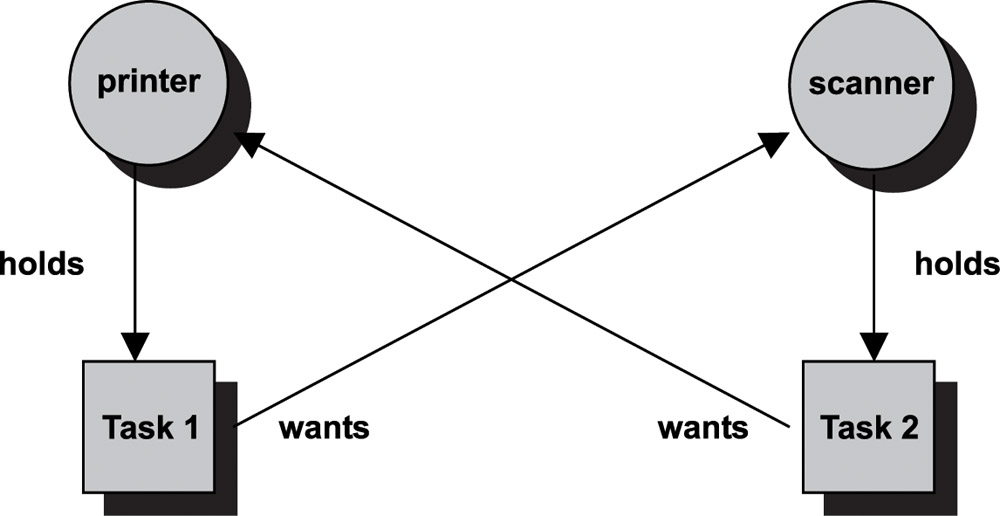
\includegraphics[width=1\textwidth]{figures/deadlock1.jpg}}
	\caption{Gambar Deadlock}
	\label{Gambar}
	\end{figure}
      
      Gambar \ref{Gambar_Deadlock} Contoh gambar pada saat terjadinya deadlock.

\subsection {Masalah Deadlock dan Metode Penanganan Deadlock}
\subsubsection {Masalah Deadlock}
	Deadlock merupakan dampak pengaruh dari sinkronisasi, yaitu dimana satu variabel yang digunakan oleh dua proses yang berbeda. Deadlock selalu tidak terlepas dari yang namanya sumber daya, karena hampir secara keseluruhan merupakan masalah mengenai sebuah sumber daya yang digunakan secara bersamaan. Sebuah Kelompok Proses yang diblok atau diblokir, dimana setiap proses memegang sebuah resource dan kemudian menunggu resource lain dari proses yang berada didalam proses yang sedang diBlok tersebut, biasanya dari semua proses-proses atau resource yang non preemptive.
	
\subsubsection {Metode Penanganan}
	Ada tiga Metode penanganan Deadlock:
	Yang Pertama yaitu, anda harus menggunakan satu protokol yang dapat membuat anda yakin bahwa sistem tersebut tidak akan pernah mengalami kejadian deadlock. Metode ini bisa disebut dengan Deadlock Prevention atau Avoidance.
	
	Yang Kedua, anda harus memberikan izin sistem untuk mengalami kejadian deadlock, namun setelah terjadinya deadlock anda harus dengan cepat segera untuk memperbaiki sistem yang mengalami deadlock tersebut. Metode ini biasanya disebut dengan Deadlock detection and recovery.
	
	Dan yang terakhir, anda hanya mengabaikan semua permasalahan yang terjadi secara bersamaan, dan kemudian menganggap bahwa deadlock tidak akan terjadi, metode ini digunakan dalam berbagai sistem operasi komputer, termasuk windows dan unix.

\begin{table}[H]
\begin{tabular}{|c|c|c|c|c|}
hline
Proses & Jumlah Sumber Daya Digenggam & Maksimum Sumber Daya Dibutuhkan\\
\hline
X   & 2 & 10\\
Y   & 1 & 3\\
Z   & 3 & 7\\
\hline
Tersedia 4
\hline
\end{tabular}
\end{table}

\subsection {Deadlock Detection}
\begin {enumerate}
\item
1. Pendeteksian secara Algoritma, yaitu dengan cara kita mengetahui jika terjadinya deadlock, deadlock terjadi jika suatu permintaan tidak dapat ditangani segera.
	
\item
2. Recovery atau Pemulihan, yaitu yang pertama menggagalkan semua proses deadlock, yang kedua mem backup semua proses yang deadlock dan kemudian silahkan melakukan restart di semua proses yang sedang terjadi, yang ketiga menggagalkan semua proses yang deadlock secara berurutan sehingga tidak akan terjadi lagi deadock, dan yang terakhir yaitu menggagalkan pengalokasian resource secara berurutan hingga tidak ada deadlock.

\end {enumerate}

\subsection {Beberapa hal yang terjadi ketika mendeteksi adanya deadlock}
\begin {enumerate}
\item
1. Permintaan sumber daya dikabulkan selama memungkinkan.
\item
2. Sistem operasi melakukan scanning apakah ada kondisi circular wait secara peiodik.
\item
3. Pemeriksaan dilakukan setiap ada sumber daya yang hendak digunakan.
\item
4. memeriksa dengan algoritma tertentu.
\end {enumerate}

\subsection {Beberapa jalan untuk kembali dari deadlock}
\begin {enumerate}
\item
1. Lewat Preemption, yaitu dengan jauhkan sumber daya dari pemakainya untuk sementara waktu, tujuannya untuk memberikannya pada proses lain. strategi dengan memberikannya kesempatan pada proses lain dengan tanpa diketahui oleh pemilik dari sumber daya itu dan tergantung juga dari sifat sumber daya itu sendiri.
\item
2. Lewat melacak kembali, setelah melakukan prosesn dari preemption tersebut maka secara otomatis proses utama yang diambil sumber dayanya akan stop dan tidak akan melanjutkan prosesnya, oleh karena itu dibutuhkan langkah untuk dapat kembali pada keadaan aman, tetapi untuk menentukan keadaan aman tersebut sangatlah susah.
\item
3. Mematikan proses yang menyebabkan deadlock, ini merupakan cara yang sangat umum digunakan yaitu dengan cara mematikan semua proses yang mengalami deadlock.
\item
4. Menghindari deadlock, pada sistem permintaan untuk sumberdaya biasanya hanya dilakukan sekali saja, sistem harus sudah dapat mengenali bahwa sistem itu aman atau tidak.
\end {enumerate}

\subsection {Reference}

@article{siahaan2015penyelarasan,
  title={Penyelarasan Pada Masalah Dining Philosophers Menggunakan Algoritma Lock \& Release},
  author={Siahaan, Andysah Putera Utama},
  journal={TECHSI-Jurnal Teknik Informatika},
  volume={7},
  number={1},
  year={2015}
}

@article{fauzi2013perangkat,
  title={PERANGKAT LUNAK VISUALISASI PERJALANAN KERETA API DENGAN MENGGUNAKAN PENDEKATAN SEMAPHORE, DEADLOCK SOLUTION DAN ALGORITMA DIJKSTRA},
  author={Fauzi, Esa},
  year={2013},
  publisher={Universitas Widyatama}
}

@book{silberschatz2014operating,
  title={Operating system concepts essentials},
  author={Silberschatz, Abraham and Galvin, Peter Baer and Gagne, Greg},
  year={2014},
  publisher={John Wiley \& Sons, Inc.}
}


%\chapter[Internet]
%{Definisi\\ Internet}
%\input{section/1internet.tex}

%\chapter[Web]
%{Definisi\\ Web}
%\input{section/1web.tex}

%\chapter[Backend]
%{Definisi\\ Backend}
%\input{section/1Backend.tex}

%\chapter[Frontend]
%{Definisi\\ Frontend}
%\input{section/1Frontend.tex}

% contoh aplikasi web service
% web service
% protokol
% port

% HTTP
% URL
% POST
% GET


\bibliographystyle{IEEEtran}
\bibliography{references, kelompok31A}

\printindex

\end{document}

